%%%%%%%%%%%%%%%%%%%%%%%%%%%%%%%%%%%%%%%%%%%%%%%%%%%%%%%%%%%%%%%%%%%%%%%%
%                                                                      %
% LaTeX, FIIW thesis template                                          %
%                                                                      %
%%%%%%%%%%%%%%%%%%%%%%%%%%%%%%%%%%%%%%%%%%%%%%%%%%%%%%%%%%%%%%%%%%%%%%%%
\documentclass[11pt,a4paper]{report}
% Indien je je thesis recto-verso wil afdrukken gebruik je onderstaande opties i.p.v. bovenstaande
%\documentclass[11pt,a4paper,twoside,openright]{report}

\usepackage[a4paper,left=3.5cm, right=2.5cm, top=3.5cm, bottom=3.5cm]{geometry}
\usepackage[dutch]{babel}
\usepackage{graphicx}
\usepackage[latin1]{inputenc}           % om niet ascii karakters rechtstreeks te kunnen inputten
%\usepackage[utf8]{inputenc}            % commentarieer deze regel uit als je utf8 encoded files gebruikt in plaats van latin1
\usepackage{natbib}
\usepackage{listings}             		% voor het weergeven van broncode
\usepackage{verbatim}					% weergeven van code, commando's, ...
\usepackage{hyperref}					% maak PDF van de thesis navigeerbaar
\usepackage{url}						% URL's invoegen in tekst met behulp van \url{http://}
\usepackage[small,bf,hang]{caption}     % om de captions wat te verbeteren
\usepackage[final]{pdfpages}            % gebruikt voor het invoegen van het artikel in pdf-formaat
\usepackage{pslatex}					% andere lettertype's dan de standaard types
\usepackage{lipsum}
\usepackage{sectsty}					% aanpassen van de fonts van sections en chapters
%\usepackage[nottoc,numbib]{tocbibind}	% Bibliography mee in de ToC
\usepackage{wrapfig}
\usepackage{mathtools}
\usepackage{amsmath}
\usepackage{pythonhighlight}
\allsectionsfont{\sffamily}
\chapterfont{\raggedleft\sffamily}

\usepackage{float}                      % De optie H voor de plaatsing van figuren op de plaats waar je ze invoegt. bvb. \begin{figure}[H]
%\usepackage{longtable}					% tabellen die over meerdere pagina's gespreid worden
%\usepackage[times]{quotchap}           % indien je fancy hoofdstuktitels wil
%\usepackage[none]{hyphenat}
%\usepackage{latexsym}
%\usepackage{amsmath}
%\usepackage{amssymb}
\hyphenation{TensorFlow}
\hyphenation{PyTorch}
\hyphenation{FlatBuffer}
\hyphenation{Python}
\hyphenation{Torchscript}
\hyphenation{ONNX}
\hyphenation{ResNet}
\hyphenation{YOLO}
\hyphenation{MMDetection}
% MFA: zet zoekpad voor figure
\graphicspath{{fig/}}

\usepackage{fiiw}
% \usepackage{fiiw_eng} % For the english version (also change last page at the bottom of this file!

%door onderstaande regels in commentaar te zetten, of op false, kan je pagina's weglaten
%bijvoorbeeld het weglaten van een voorwoord, lijst met symbolen, ...
%%%%%%%%%%%%%%%%%%%%%%%%%%%%%%%%%%%%%%%%%%%%%%%%%%%%%%%%%%%%%%%%%%%%%%%%%%%%%%%%%%%%%%%%
%voorwoord toevoegen?
\acknowledgementspagetrue
\acknowledgements{voorwoord}			%.tex file met daarin het voorwoord

%samenvatting toevoegen
\summarypagetrue
\summary{summary}					%.tex met daarin de samenvatting

%abstract toevoegen?

\abstractpagetrue
\abstracts{abstract}					%.tex file met daarin het abstract
%lijst van figuren toevoegen?
\listoffigurespagetrue
%lijst van tabellen toevoegen?
\listoftablespagetrue
%lijst van symbolen toevoegen?
%\listofsymbolspagetrue
%\listofsymbols{symbolen}				%.tex file met daarin de lijst van symbolen
%lijst van afkortingen toevoegen?
\listofabbrevspagetrue
\listofabbrevs{afkortingen}				%.tex file met daarin de lijst van symbolen

%informatie over het eindwerk, de promotor, ...
%%%%%%%%%%%%%%%%%%%%%%%%%%%%%%%%%%%%%%%%%%%%%%%
\opleiding{Elektronica-ICT}
\afdeling{ICT}

\campus{denayer} %denayer,denayereng,geel,geeleng,gent,ghenteng,groept,groupteng,brugge,brugeseng

% onder embargo? laat leeg indien van niet; vul de datum in als dd-mm-yyyy indien van wel
\embargo{}

\title{Mobile Deep Visual Detection and Recognition}
\subtitle{}
% \author{naam student}
\forenameA{Thijs}
\surnameA{Vercammen}
\forenameB{}
\surnameB{}

\academicyear{2021 - 2022}

\promotorA[Promotor]{Prof. dr. ir. Toon Goedem\'e}
\promotorB[Co-promotor]{Ing. Floris De Feyter}

\begin{document}
\selectlanguage{dutch}
% \selectlanguage{english} % For the english version
\preface

%%%%%%%%%%%%%%%%%%%%%%%%%%%%%%%%%%%%%%%%%%%%%%%%%%%%%%%%%%%%%%%%%%% 
%                                                                 %
%                            CHAPTER                              %
%                                                                 %
%%%%%%%%%%%%%%%%%%%%%%%%%%%%%%%%%%%%%%%%%%%%%%%%%%%%%%%%%%%%%%%%%%% 

%\chapter{Vormelijke richtlijnen van de scriptie}
\chapter{Situering en doelstelling}

\section{Situering}
Tegenwoordig wordt deep learning steeds meer en meer gebruikt om beeldverwerking problemen op te lossen. Via neurale netwerken kunnen we met meer en betere features werken om de afbeeldingen te analiseren. Maar veel van deze modelen hebben behoorlijk wat rekenkracht en geheugen nodig om te werken. Ook is er steeds meer intresse naar real-time toepassingen waarvan het resultaat zo snel mogelijk beschikbaar moet zijn. Dit wordt moeilijk bij veel hedendaagse systemen waarbij de foto eerst genomen moet worden en vervolgens door een computer geanaliseerd moet worden, omdat hedendaagse systemen veel rekenwerk en geheugen vragen. In deze masterproef wordt er onderzocht of de computer kan weggelaten worden en de afbeelding meteen door het mobiel apparaat geanaliseerd kan worden. Dus er moet onderzocht worden hoe een bestaand model aangepast kan worden om effici\"ent te werken op een mobiel apparaat. Hierbij moet vooral rekening gehouden worden met de rekenkracht en geheugen van het mobiele apparaat.

\section{Probleemstelling}
Mobiele apparaten zijn kleine toestellen met beperkt geheugen en beperkte rekenkracht. In deze masterproef wordt er onderzocht hoe het rekenwerk beperkt kan worden zodat het resultaat real-time geleverd kan worden. Er gaat ook onderzocht worden hoe alle data effici\"ent kan worden opgeslagen op het toestel. 

\section{Doelstellingen}
Het uiteindelijke doel van deze masterproef is er voor zorgen dat een bestaand deep learning model aangepast kan worden zodat dit real-time resultaten kan geven op een mobiel apparaat. Dit gebeurt aan de hand van de volgende stappen:
\begin{itemize}
    \item grondig begrijpen van een deep learning herkenningssysteem
    \item grondig begrijpen van een deep learning detectiesysteem
    \item Onderzoeken welke technieken er gebruikt kunnen worden om bestaande systemen op een mobiel apparaat te implementeren.
    \item onderzoeken voor optimalisaties voor een herkenningssysteem
    \item onderzoeken voor optimalisaties voor een detectiesysteem
    \item gevonden technieken testen en analiseren
    \item werkend prototype applicatie ontwerpen voor een mobiel apparaat
\end{itemize}
%%%%%%%%%%%%%%%%%%%%%%%%%%%%%%%%%%%%%%%%%%%%%%%%%%%%%%%%%%%%%%%%%%% 
%                                                                 %
%                            CHAPTER                              %
%                                                                 %
%%%%%%%%%%%%%%%%%%%%%%%%%%%%%%%%%%%%%%%%%%%%%%%%%%%%%%%%%%%%%%%%%%% 
%\chapter{Structuur van de masterproeftekst}
\chapter{Herkenning en Detectie Algemeen}

\section{Deep learning-gebaseerde herkenningssystemen}
Herkenningssystemen voorspellen wat de identiteit is van een afbeelding. 
Dit is het herkennen van objecten in digitale afbeeldingen zonder deze te lokaliseren of aan te duiden. 
Bij herkenningssystemen is er geen of weinig overlap tussen de trainingsafbeeldingen en de inputafbeeldingen.
Bijvoorbeeld bij gezichtsherkenning wordt er een algemeen herkenningssysteem ontworpen dat gezichten herkent, en niet een systeem dat elk individueel gezicht herkent.
Voor een herkenningssysteem is er een goed getraind neuraal netwerk nodig dat een input afbeelding omzet in features. 
Er moet een database zijn met daarin de gegevens van de objecten die men wil herkennen. 
Vervolgens is er ook een methode nodig om features van het neuraal netwerk te vergelijken met de gegevens in de database om het juiste object te herkennen.

\subsection{Herkenning}
Wanneer er een getraind neuraal netwerk aanwezig is kan er een herkenningssysteem ontwikkeld worden. 
Als men een bepaald object in een afbeelding wil herkennen gaat men met behulp van een neuraal netwerk de afbeelding omzetten in een embedding. 
Volgens \cite{koehrsen_neural_2018} zijn embeddings vectoren die kunnen worden vergeleken in een embedding space, waar gelijkaardige objecten dichter bij elkaar liggen. 
De embedding van de input afbeelding wordt vergeleken met de embeddings die zich in een galerij bevinden. 
\cite{jiang_deep_2019} vermeldt dat met behulp van een query er gelijkaardige objecten uit de galerij gehaald kunnen worden om deze vervolgens te gaan vergelijken in een embedding space. 
Deze galerij is een database/verzameling met gekende embeddings/ID's van de objecten die men wil herkennen.
Een query is een embedding van de input waarvan het label niet gekend is.
Gelijkaardige embeddings kunnen gezocht worden via de nearest neighbour techniek.
De nearest neighbour techniek vermeld in \cite{8010421} gaat in de embedding space kijken naar het K-aantal dichtste buren van een query.
Het label dat het meest voorkomt tussen het K-aantal buren, zal dan ook het meest waarschijnlijke label zijn voor de query.
Figuur \ref{fig:embedding} is een voorbeeld van een embedding space, een query is een punt in deze grafiek dat nog geen label heeft.
Voor het herkennen van een afbeelding gaan we in de grafiek naar de K dichtsbijzijnde buren kijken van de query.

\begin{figure}[!ht]
    \centering
 	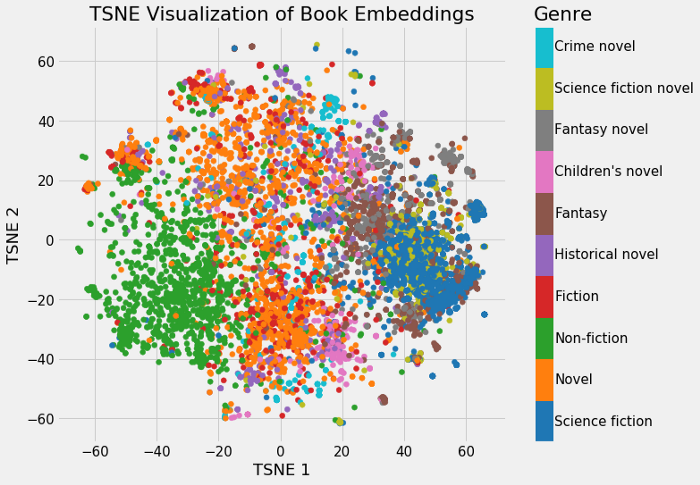
\includegraphics[width=0.7\linewidth]{fig/embedding.png}
 	\caption{Voorbeeld van embedding space voor boek genres.}
	\cite{koehrsen_neural_2018}
 	\label{fig:embedding}
\end{figure}

\subsection{Convolutioneel neuraal netwerk (CNN) }
De belangrijkste bouwsteen van een herkenningssysteem is een getraind CNN.
In deze paragraaf bespreken we het CNN en zijn verschillende bouwstenen beschreven door \cite{jiang_deep_2019}.
Figuur \ref{fig:cnn} is een voorbeeld van een CNN en zijn verschillende onderdelen.

\begin{figure}[!ht]
    \centering
 	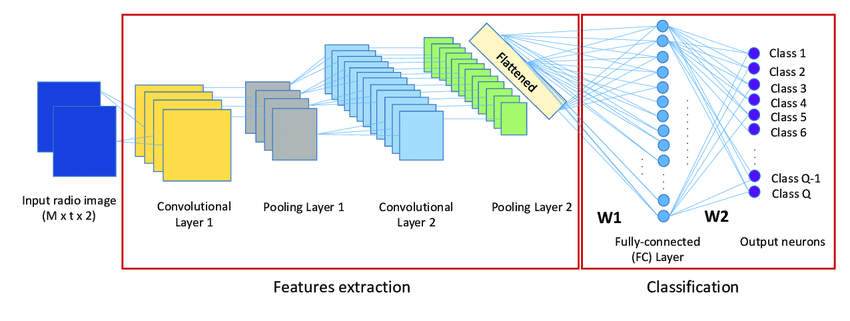
\includegraphics[width=0.85\linewidth]{fig/cnn_2.png}
 	\caption{CNN met twee convolutie lagen en twee pooling lagen en \'e\'en fully-connected laag}
 	\label{fig:cnn}
	 \cite{s19143127}
\end{figure}
 
Het belangrijkste deel van een CNN zijn de convolutielagen (figuur \ref{fig:conv_laag}). 
Bij een convolutielaag wordt een kernel/filter over de input geschoven om features te bepalen. 
Een kernel bestaat uit een set van waardes die we gewichten noemen.
Op elke plaats waar deze kernel voorbijkomt vermenigvuldigen we de gewichten met de input.
Deze actie wordt de convolutie genoemd.
Alle pixels binnen het veld van de kernel worden gereduceerd tot een enkele waarde. 
De convoluties zijn zeer effici\"ent om visuele informatie uit de input te halen.
Convolutielagen leren verschillende features door meerdere kernels in parallel uit te voeren per convolutielaag. 
Dit zorgt ervoor dat de matrices met featuremappen per kernel steeds kleiner worden maar ook dieper worden. 
Een andere factor van een convolutie laag is de stride.
Deze waarde geeft aan met hoeveel pixels de kernel telkens moet doorschuiven. 
Als de stride \'e\'en is dan schuift de kernel steeds op met \'e\'en pixel en als de stride drie is dan schuift de kernel op met drie pixels.
Stride \'e\'en zorgt voor meer features per featuremap, maar maakt het CNN trager omdat er meer bewerkingen moeten worden uitgevoerd.
Een CNN bestaat uit een opeenvolging van een aantal convolutielagen die steeds meer high-level features extraheren. 
Hoe meer convolutielagen een netwerk telt hoe meer features er uit de input worden gehaald, maar hoe trager het netwerk is. 

\begin{figure}[!ht]
	\centering
	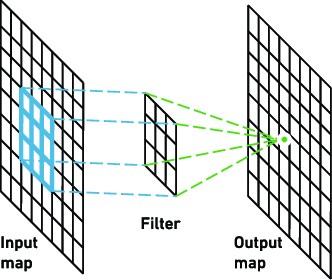
\includegraphics[width=0.35\linewidth]{fig/convolution layer.png}
	\caption{Convolutielaag waarbij de input vermenigvuldigd wordt met een kernel. De vermenigvuldigde inputwaardes worden vervolgens herleid tot een enkele waarde. Vervolgens zal de filter opschuiven en opnieuw deze actie uitvoeren.}
	\label{fig:conv_laag}
	\cite{brownlee_convolutional_2017}
\end{figure}

Na elke convolutielaag komt een niet lineaire activatie functie.
De niet lineare activatie functie zorgt ervoor dat het CNN niet herleid kan worden tot \'e\'en convolultielaag die geen high-level features kan extraheren. 
De meest gebruikte functie hiervoor is de rectified linear unit (ReLu) (figuur \ref{fig:relu}). 
De ReLu wordt vaak gebruikt omdat deze veel sneller wordt uitgevoerd dan andere activatie functies zoals Sigmoid en Tangens hyperbolicus (\cite{Krizhevsky_act_2017}).
De ReLu kan exact 0 weergeven en ziet er lineair uit. 
Max(0,x) is de ReLu bewerking, dus er wordt verdergegaan met 0 of de input waarde. 
%sigmoid en tanh sitaat

\begin{figure}[!ht]
 	\centering
 	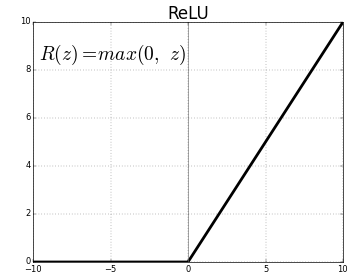
\includegraphics[width=0.35\linewidth]{fig/ReLu.png}
 	\caption{ReLu, waarbij het maximum wordt genomen van 0 en de input waarde.}
 	\label{fig:relu}
	\cite{Kanchan_activation_2018}
\end{figure}

Een volgende bouwsteen is de poolinglaag.
Deze laag vermindert het aantal features per feature map. 
De meest voorkomende methode is max-pooling weergegeven in figuur \ref{fig:maxpool} waarbij er verder wordt gegaan met de maximum waarde in een bepaalde regio. 
Het doel van een poolinglaag is om het aantal parameters te verminderen en zo ook het rekenwerk te verminderen. 
Er kan ook gebruik gemaakt worden van avarage pooling waarbij er verder wordt gegaan met de gemiddelde waarde van een regio. 
Er is ook minimal pooling waarbij er verder wordt gegaan met de minimum waarde.

\begin{figure}[!ht]
	\centering
	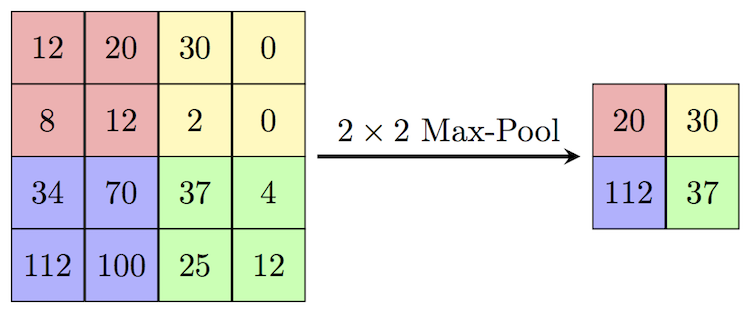
\includegraphics[width=0.5\linewidth]{fig/Maxpool.png}
	\caption{Maxpooling waarbij er verder wordt gegaan met de maximum waarde in een 2x2 regio.}
	\label{fig:maxpool}
\end{figure}

Op het einde van elk CNN volgen er meestal \'e\'en of meerdere fully connected lagen. 
Deze lagen connecteren elke input van \'e\'en laag met elke activatie eenheid van de volgende laag, dit is weergegeven in het classificatie gedeelte van figuur \ref{fig:cnn}. 
Dit zorgt voor meer parameters en meer rekenwerk, maar ook voor meer features.
Door het extra rekenwerk vormen deze lagen een vertragende factor. 
De fully connected lagen zorgen voor een classificatie op basis van de features van de convolutie lagen.

\subsection{Trainen van een CNN} \label{train}
Het trainen van een CNN bestaat uit het leveren van veel afbeeldingen met labels aan het netwerk. 
Op basis van het resultaat van deze voorbeelden worden de gewichten van de kernels telkens aangepast.
Zo levert het CNN steeds een beter resultaat. 

Tijdens het trainen van een CNN nemen we een groep met trainingsafbeeldingen en geven we deze als input aan het CNN.
Het CNN geeft een voorspelling van deze trainingsafbeelding.
Vervolgens vergelijken we de voorspelling met de label van de trainingsafbeelding.
Per groep trainingsafbeeldingen wordt er via een loss functie het verschil tussen de voorspelde waarde en de werkelijke waarde berekend.
De loss functie geeft de error van de voorspelling weer tijdens het trainen van een neuraal netwerk. 
Als al de groepen met trainingsafbeeldingen \'e\'en keer zijn gebruikt als trainingsinput dan is er \'e\'en epoch voltooid.
Zo kan het CNN X-aantal epochs uitvoeren waarbij de trainingsafbeelding X-aantal keer door het CNN worden verwerkt.

De stochastic gradient descent is een techniek die men gebruikt om de loss van het CNN te minimaliseren.
Hierbij wordt op basis van de loss functie de gradi\"ent voor elk gewicht berekend door de afgeleide te nemen van de loss naar dit gewicht.
\begin{equation}
	\textrm{gradient}  = \frac{\partial \textrm{loss}}{\partial \textrm{gewicht}}
\end{equation}
Via de berekende gradi\"enten kunnen we nu de gewichten aanpassen zodat de loss geminimaliseerd wordt.
We kunnen de factor waarmee we de gewichten aanpassen be\"invloeden met de learning rate.
De learning rate is een factor die aangeeft hoe groot de stap moet zijn waarmee de gewichten worden aangepast.
\begin{equation}
	\textrm{gewicht} = \textrm{oud\_gewicht} - (\textrm{learning rate} * \textrm{gradient})
\end{equation}
Hoe kleiner de learning rate hoe langer het trainen van een CNN duurt.
Een te grote learning rate kan echter resulteren in een slecht getraind netwerk, omdat de veranderingen op de gewichten dan te groot zijn om een beter resultaat te krijgen.

\subsection{Transfer Learning}
Bij transfer learning (\cite{Geiger_IJRR_2013}) wordt er verder gebouwd op een model dat reeds getraind is.
Hierbij maakt men gebruik van een basismodel waarvan de toepassing gerelateerd is aan de gewenste toepassing.
Bijvoorbeeld een model waarmee we dieren kunnen herkennen gebruiken we als basis voor een model dat hondenrassen herkent.
Op dit basismodel kan er verder getraind worden met een dataset specifiek voor de gewenste toepassing.
Deze dataset kan veel kleiner zijn dan een dataset die nodig is om een nieuw model te trainen.
Het trainen van een nieuw CNN kan soms weken duren.
Via transfer learning kan de trainingsperiode met een grote factor gereduceerd worden.
Deze methode gebruiken we voornamelijk om een 'nieuw' model te trainen vanwege de kleinere trainingsdataset en kortere trainingstijd.

\subsection{ResNet50} \label{resnet}
Het herkenningsnetwerk dat we willen implementeren in deze masterproef is de ResNet50 architectuur.
\cite{he2015deep} hebben vastgesteld dat als het aantal lagen van een CNN toeneemt dat op een bepaald moment de training accuraatheid daalt.
%Dit verschijnsel noemt men de vanishing gradient.
In paragraaf \ref{train} hebben we besproken hoe we de gradi\"ent kunnen berekenen tijdens het trainen van een CNN.
Voor elke laag in het CNN moet de gradi\"ent opnieuw berekend worden door telkens opnieuw de afgeleide te berekenen.
Hierdoor wordt de gradient steeds kleiner en kleiner tot deze een minimum bereikt.
Waardoor de gewichten in de eerste lagen zich heel traag aanpassen of zelfs niet meer veranderen.
\cite{he2015deep} die dit probleem hebben vastgesteld hebben dit opgelost door gebruik te maken van skip connections.
Hierbij wordt de input van een laag rechtstreeks met een volgende laag geconnecteerd die x aantal lagen verder ligt.
Op deze manier worden de gradi\"enten per laag niet meer kleiner.
%ResNet50  lagen waarbij er een skip connection plaatsvindt per 3 lagen.
De ResNet50 architectuur bestaat uit 50 convoluties en is opgebouwd uit ResNet blokken die bestaan uit 3 convolutie lagen en 1 skip connection.

\begin{figure}[!ht]
	\centering
	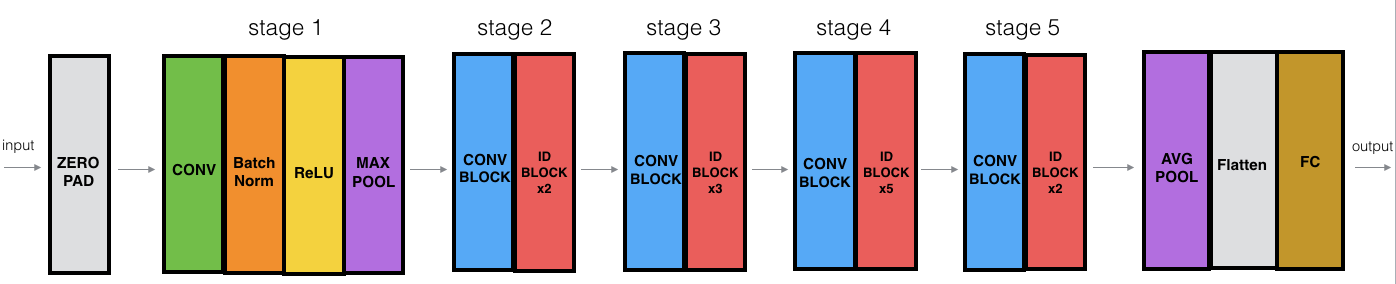
\includegraphics[width=1.0\linewidth]{fig/resnet50.png}
	\caption{ResNet50 architectuur met de al de operaties. Ook zijn er 2 verschillende ResNet blokken terug te vinden het convolutieblok en het ID-blok.}
	\label{fig:resnet}
	\cite{Raghunandepu_resnet_2019}
\end{figure}

In figuur \ref{fig:resnet} is het standaard ResNet50 netwerk te zien.
In deze figuur kunnen we de voornaamste operaties terug vinden die in het netwerk gebruikt worden.
Ook vinden we in deze architectuur twee verschillende ResNet blokken terug: de ID-blok en de convolutie blok.
In figuur \ref{fig:resnet_b} zien we de twee verschillende blokken en hun operaties weergegeven.
De bovenste blok is de ID-blok, dit is de standaard ResNet50 blok waarbij de input en output dimensies gelijk zijn.
De onderste blok in deze afbeelding is het convolutieblok waarbij twee extra operaties worden uitgevoerd tijdens de skip connections.
Deze twee extra operaties zijn nodig als de input en output dimensies van het ResNet50 blok verschillend zijn.

\begin{figure}[!ht]
	\centering
	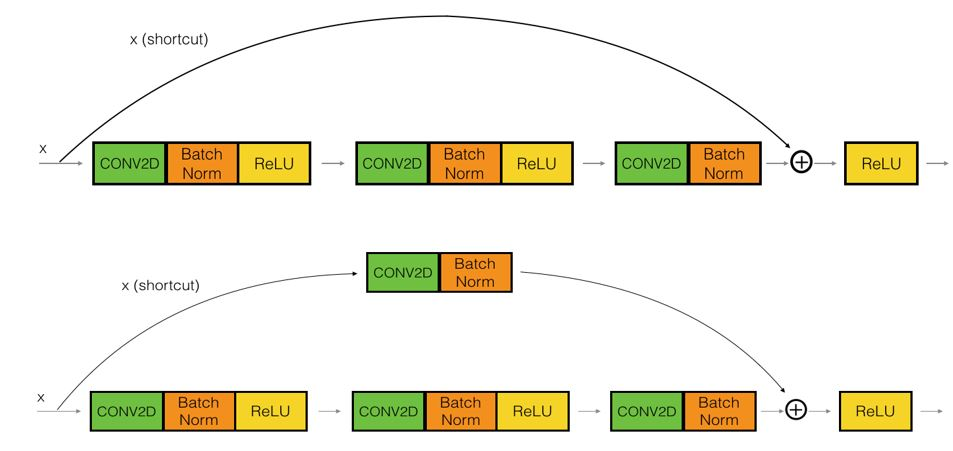
\includegraphics[width=1.0\linewidth]{fig/resnet_blokken.jpg}
	\caption{De bovenste blok is de ID blok van de ResNet50 architectuur. De onderste is de Convolutieblok van de ResNet50 architectuur}
	\label{fig:resnet_b}
	\cite{Raghunandepu_resnet_2019}
\end{figure}

\section{Deep learning-gebaseerde detector}
Objectdetectie is het lokaliseren en classificeren van objecten in een afbeelding, waarbij de objecten aangeduid worden met een bounding box.
Een bounding box is een kader die rond een object wordt getekend. 
De klassieke versie van objectdetectie is de sliding window benadering.
Waarbij een venster met vaste grootte over de afbeelding schuift en telkens de gegevens binnen het venster analyseert.
Momenteel kan objectdetectie worden opgedeeld in twee methodes: de single-stage detector en de two-stage detector.

\subsection{Two-stage detector}
Two stage detectoren focussen op accuraatheid ten koste van de uitvoeringssnelheid.
Zoals de naam zegt bestaat deze methode uit twee niveaus. 
In het eerste niveau worden er Regions of Intrest (RoIs) gecre\"eerd.
Dit is het filteren van regio's waarbij de kans groot is dat deze een object bevatten. 
Het tweede deel classificeert en verfijnt de lokalisatie van de RoIs die in het eerste deel gecre\"eerd werden. 

De voornaamste two-stage detector is de Faster R-CNN detector \cite{ren_faster_2016}. 
Hierbij wordt via een CNN, die de backbone wordt genoemd, eerst de features uit de afbeelding gehaald.
Deze backbone is meestal een standaard herkenningsnetwerk zoals ResNet50 maar dan zonder de classificatielagen.

Vervolgens wordt er gebruik gemaakt van een Region Proposal Network (RPN) weergegeven in figuur \ref{fig:faster-r-cnn}. 
Het RPN is een volledig convolutioneel netwerk dat regio's uit de afbeelding filtert waar de kans groot is dat er objecten opstaan.
Per input geeft het RPN een set van regio's als output.
Elk van deze regio's heeft een objectness score wat aangeeft in welke mate de regio een object bevat.
Om een region proposal te genereren wordt het RPN over de feature map geschoven dat gegenereerd is door de backbone.
Op elke sliding window locatie van het RPN worden er meerdere regio voorspellingen gedaan.
Deze voorspelling doet het RPN door verschillende anchor boxes te evalueren per sliding window locatie.
Anchor boxes zijn een vooraf gedefini\"eerde set van bounding boxes met drie verschillende vormen in drie verschillende schalen.
Via de non-maxima supression methode zorgen we ervoor dat er maar \'e\'en anchor box overblijft van de overlappende anchor boxes. 
Deze techniek houdt enkel de anchor box over met de beste voorspelling en onderdrukt de rest van de anchor boxes.

Na het RPN komt de RoI Pooling laag.
Deze laag gebruikt max-pooling om de feature map van elke RoI om te zetten naar een feature map met vaste grootte.
Elk van deze features gaat door een set van fully connected lagen die twee lagen als output heeft.
Een softmax laag die de klasse voorspelt en een bounding box regressie laag die de bounding box voorspelt.
%dieper ingaan op softmax en bbox voorspelling

\begin{figure}[!ht]
    \centering
 	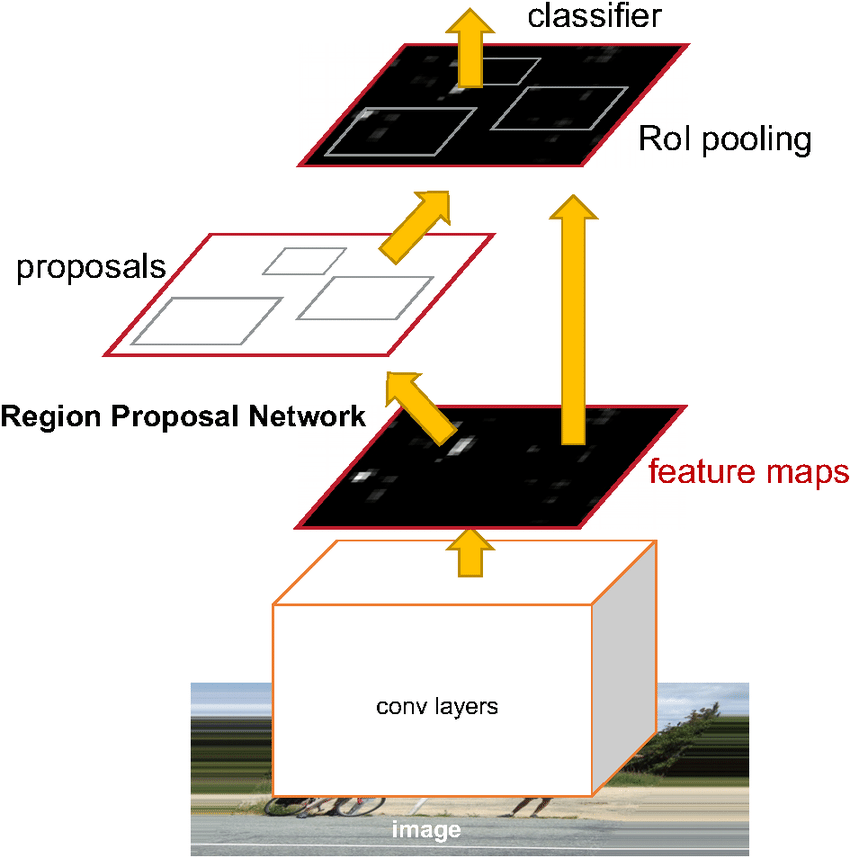
\includegraphics[width=0.35\linewidth]{fig/Faster-R-CNN.png}
 	\caption{Faster R-CNN}
 	\label{fig:faster-r-cnn}
	\cite{ren_faster_2016}
\end{figure}

\subsection{One-stage detector}
Bij one-stage detectoren gebeurt objectdetectie in \'e\'en keer. 
Dus er is geen region proposal niveau meer zoals bij de two-stage detector. 
Deze detectoren gebruiken minder geheugen en rekenkracht dan two-stage detectoren.
Maar deze detectoren kunnen in nauwkeurigheid verliezen t.o.v. two-stage detectoren.
Deze detectoren zijn zeer geschikt om gebruikt te worden op mobiele apparaten, omdat deze detectoren sneller zijn en minder geheugen nodig hebben.
Twee veel gebruikte technieken van one-stage detectie zijn: You Only Look Once (YOLO) en Single Shot Detection (SSD).

\begin{figure}[!ht]
	\centering
	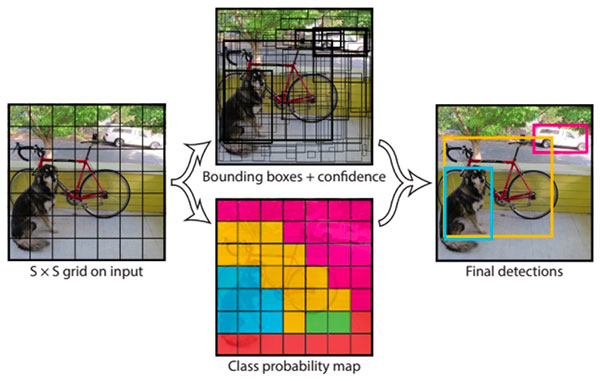
\includegraphics[width=0.60\linewidth]{fig/YOLO.jpg}
	\caption{YOLO waarbij de input is opgedeeld in een S x S rooster. 
	En waarbij bounding box voorspellingen zijn gedaan.}
	\label{fig:yolo}
	\cite{redmon_you_2016}
\end{figure}

YOLO \cite{redmon_you_2016} verdeelt de afbeelding in een S x S rooster zoals in figuur \ref{fig:yolo} te zien is. 
De cel waarin het middelpunt van het object valt is verantwoordelijk voor de object detectie.
Elke cel zal bounding boxes voorspellen en een zekerheid score bepalen voor elke bounding box. 
Deze score geeft aan hoe zeker het model is dat een bepaalde bounding box een object bevat.
Elke cel in het rooster kan meerdere bounding boxes voorspellen.
Per cel wordt ook de klasse van het object voorspelt.

%Deze score wordt bepaalt met de Intersection Of Union (IOU) tussen de voorspelde box en de ground truth box.
%IOU
De YOLO detector kan voor elke cel meerdere bounding boxen voorspellen voor een enkel object.
Om \'e\'en bounding box per object te krijgen zullen we eerst alle bounding boxen waarvan de score onder een bepaalde drempel ligt moeten verwijderen.
Vervolgens passen we Non-maxima supression toe om de overbodige bounding boxen te verwijderen. 
%Een eerste mogelijkheid is door enkel bounding boxen te bepalen waarvan de voorspelling boven een zekere treshold ligt. 
Zoals de naam van de techniek zegt, worden bounding boxen die niet maximaal zijn onderdrukt.
Op deze manier blijft enkel de optimale bounding box over.
%Een andere methode is non-maxima supression, een methode die ervoor zorgt dat elk object maar \'e\'en bounding box heeft. 
%Deze techniek houdt enkel de bounding box over met de beste voorspelling en onderdrukt de rest van de bounding boxes. 

%SSD \cite{liu_ssd_2016} is een one-stage detector waarbij een afbeelding door verschillende convolutielagen gaat.
%Dit resulteert in feature mappen met verschillende schalen.
%Op elke locatie van deze feature mappen wordt een vaste set van bounding boxen ge\"evalueerd.
%Voor elk van deze boxen wordt de zekerheid dat het een object bevat voorspeld.
%Op het einde wordt non maximum suppression gebruikt om de finale voorspelling te maken.
%In figuur \ref{fig:ssd} is te zien dat een SSD bestaat uit drie delen.
%De eerste twee delen bestaan uit een standaard classificatie netwerk zonder de fully-connected lagen en een set van extra convolutielagen.
%Het derde deel doet de effectieve detectie voor elke feature map met een verschillende schaal. 

%\begin{figure}[!ht]
%	\centering
%	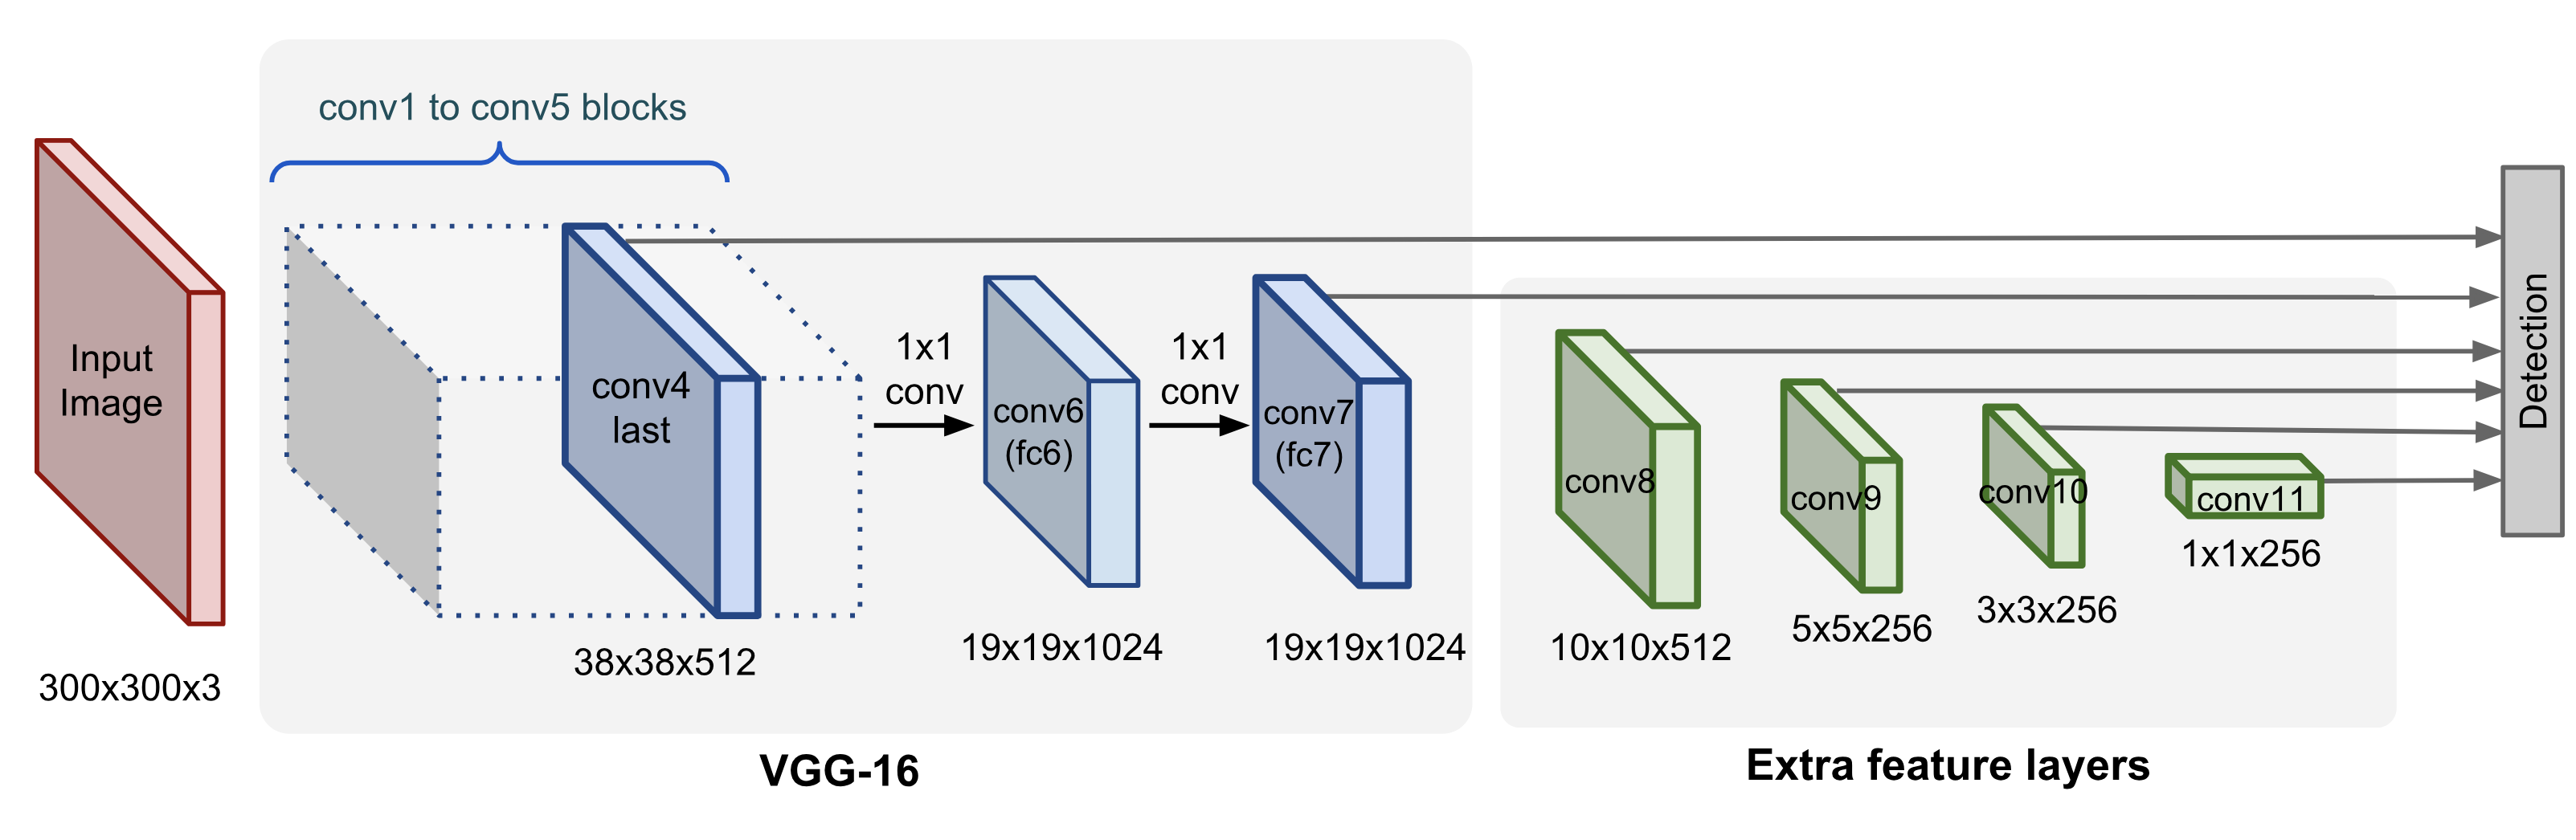
\includegraphics[width=0.80\linewidth]{fig/SSD.png}
%	\caption{One-stage detector met VGG als backbone, elke feature map met een verschillende schaal wordt ge\"evalueerd.}
%	\label{fig:ssd}
%\end{figure}
\subsection{Mean avarage precision (mAP)} \label{map}
Mean average precision besproken door \cite{Yohanandan_map_2020} is een evaluatie eenheid die gebruikt wordt om object detectoren te evalueren.
Bij deze evaluatiemethode gaan we de voorspelde bounding boxes en de classificatie evalueren.
Hierbij gaan we de precision en de recall bereken op basis van de Intersection of Union (IoU).
Bij de IoU bereken we de overlap tussen de voorspelde bounding box en de ground truth bounding box.
De ground truth bounding box is de output die we verwachten na het uitvoeren van het object detectie model.
In figuur: \ref{fig:iou} wordt weergegeven hoe we de IoU berekenen.

\begin{figure}[!ht]
	\centering
	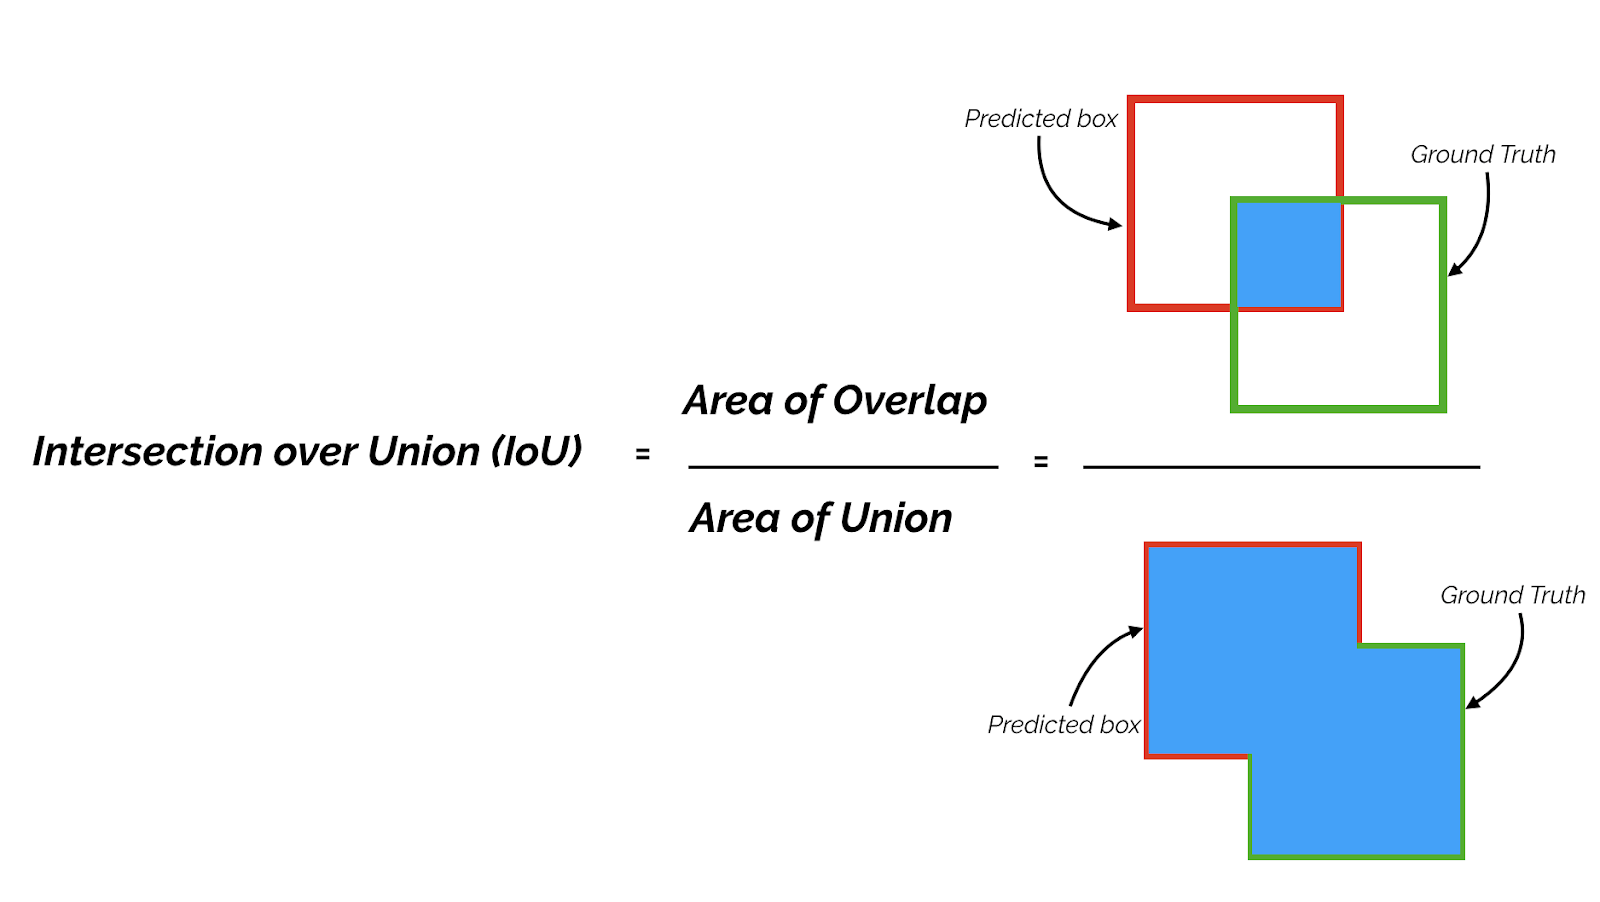
\includegraphics[width=0.80\linewidth]{fig/iou.png}
	\caption{In deze afbeelding kunnen we zien hoe de overlap/IoU wordt berekend}
	\label{fig:iou}
	\cite{Yohanandan_map_2020}
\end{figure}

Via de volgende formules kunnen we dan de precision en recall gaan berekenen.
\begin{equation}
	\textrm{Precision}  = \frac{\textrm{TP}}{(\textrm{TP} + \textrm{FP})} \qquad
	\textrm{Recall}  = \frac{\textrm{TP}}{(\textrm{TP} + \textrm{FN})}
\end{equation}

Waarbij:
\begin{itemize}
	\item TP (True Positive): wanneer IoU \textgreater treshold en de classificatie is correct.
	\item FP (False Positive): wanneer IoU \textgreater treshold en er is een foute classificatie of omgekeerd. Een voorspelling is ook FP wanneer het object meerdere keren is voorspelt.
	\item FN (False Negative): Wanneer er geen object is voorspelt terwijl er wel \'e\'en is.
\end{itemize}

Met deze gegevens kunnen we de Precision/Recall grafiek tekenen.
De oppervlakte onder deze grafiek vormt de mAP.
Om de mAP van de detectiesystemen te evalueren gaan we gebruiken maken van de Brambox tool \cite{eavise_eavise_2020}.

%%%%%%%%%%%%%%%%%%%%%%%%%%%%%%%%%%%%%%%%%%%%%%%%%%%%%%%%%%%%%%%%%%% 
%                                                                 %
%                            CHAPTER                              %
%                                                                 %
%%%%%%%%%%%%%%%%%%%%%%%%%%%%%%%%%%%%%%%%%%%%%%%%%%%%%%%%%%%%%%%%%%% 
 
\chapter{Herkenning en detectie implementatie op mobiel platform}
Dit hoofdstuk zal gaan over het implementeren van deep learning herkeningssystemen en detectiesystemen op een mobiel platform.
In dit hoofdstuk wordt er besproken welke technologi\"en er gebruikt kunnen worden om een CNN te implementeren op een mobiel platform.
Dit gaan een aantal frameworks zijn die de programeur in staat stelt om een bestaand model te implementeren op een mobiel apparaat.
Deze frameworks gaan vergeleken worden om te kijken van welk framework het best gebruik wordt gemaakt voor een bepaalde toepassing.
Er wordt ook onderzocht hoe een bestaand herkeningssystemen en detectiesystemen ge\"optimalisserd kan worden zodat dit gebruikt kan worden op een mobiel platform.
Bij het uitvoeren van een neuraal netwerk op een mobiel apparaat zal men rekening moeten houden met de volgende zaken: 
gelimiteerde rekenkracht en beschikbaar geheugen.
Ook moet er rekening gehouden worden met een beperkte batterij, want CNN's gebruiken veel bandbreedte en voeren veel berekeningen uit wat meer energie verbruikt.
Dus er zal onderzocht moeten worden welke methodes men kan gebruiken om het geheugen van het model, het aantal bewerkingen en het energieverbruik te kunnen verbeteren.
%refereren

\section{Van object detectie model naar een mobiele Implementatie}
Om machine learning modelen te ontwerpen en te trainen kan er gebruik gemaakt worden van frameworks.
Deze frameworks geven de programeur een set van tools die hun in staat stelt om op een overzichtelijke en flexibele manier machine learning modellen te ontwerpen en trainen.
In deze paragraaf worden enkele van de meest gebruikte frameworks besproken.
Dit zijn enkele van de meest gebruikte frameworks, maar zeker niet allemaal.

\section{Frameworks}
TensorFlow en PyTorch zijn de 2 voornaamste frameworks die gebruikt worden om neurale netwerken te ontwerpen en trainen.
Veel van de tools en bibliotheken die gebruikt worden om herkeningssystemen en detectiesystemen te ontwerpen worden bovenop deze frameworks gebruikt.

\subsection{TensorFlow}
TensorFlow (\cite{abadi_tensorflow_2016}) is ontworpen door Google en is een open source library voor machine learning implementaties.
TensorFlow focust op het trainen en het deployen van neurale netwerken.
Ook ondersteund TensorFlow meerdere programeer talen zoals: Python, Java en C.
Door de introductie van de Keras API is TensorFlow meer gebruiksvriendelijk geworden.
Keras is een framework dat bovenop TensorFlow gebruikt kan worden, waarmee machine learning modellen kunnen ontworpen worden op een overzichtelijke manier.
%Keras refereren
Zo heeft TensorFlow een gebruiksvriendelijk API voor eenvoudige projecten en meer uitgebreide tools voor complexe projecten.
%TensorFlow kan  dynamisch zijn grafieken wanneer variabelen worden gedeclareerd.
Door gebruik te maken van TensorBoard kan data op een flexibele manier gevisualiseerd worden tijdens runtime. 
TensorFlow biedt ook goede ondersteuning op gebied van deployment van een productie model.
Nog een voordeel van TensorFlow is dat het een grootte community achter zich heeft, omdat dit een veel gebruikt framework is.
%extra sectie voor Keras

\subsection{PyTorch}
PyTorch (\cite{li_PyTorch_2020}) is ontworpen door facebook en wordt zoals TensorFlow ook gebruikt voor machine learning implementaties.
Dit is een python gebaseerd framework dat focust op flexibiliteit, maar deze extra flexibiliteit zorgt voor meer lijnen code.
Door zijn flexibiliteit is het gemakkelijk om nieuwe functionaliteiten toe te voegen door bestaande code aan te passen of nieuwe code toe te voegen.
PyTorch maakt gebruik van externe tools zoals TensorBoard om data te visualiseren.
Dit framework wordt gebruikt om een machine learning model te ontwerpen en trainen.
Het model dat is ontworpen kan vervolgens gebruikt worden gebruikt om een applicatie te ontwerpen.
%Vermits PyTorch voornamelijk focust op het ontwerpen van netwerken zal dit in deze masterproef minder van toepassing zijn.

%vergelijking tf en PyTorch
PyTorch wordt voornamelijk gebruikt om te experimenteren met neurale netwerken.
Bedrijven en onderzoekers gebruiken dit framework vooral om een CNN experimenteel op te bouwen en te trainen.
TensorFlow wordt voornamelijk gebruikt om het model effectief in gebruik te nemen.
%De TensorFlow Lite conversie geeft meer zekerheid t.o.v. de PyToch Mobile conversie vermits deze nog in zijn Beta fase zit.

\section{Object detectie bibliotheken}
Er zijn heel wat bibliotheken die de programeur kan importeren.
Deze bibliotheken geven de programeur extra tools en hulpmiddelen om een detectiesysteem te ontwerpen en te trainen.

\subsection{MMDetection}
MMDetection maakt deel uit van OpenMMLab en is een open source object detectie toolbox gebaseerd op PyTorch.
De toolbox bevat gewichten van meer dan 200 voorgetrainde modellen.
Via modulair ontwerp kan het detectie framework opgesplitst worden in verschillende componenten.
Met de verschillende componenten kan een eigen detectie model worden gemaakt door de verschillende componenten te combineren.
MMDetection ondersteund ook 48 verschillende detectie methodes zoals: YOLO, Faster R-CNN, etc.
Al de bounding box en masker operaties worden uitgevoerd op GPU's dit geeft MMDetectie een grootte trainingssnelheid.
MMDetection biedt geen ondersteuning om een bestaand model te optimaliseren naar een model voor mobiele toepassingen.
Dus dit model zal geconverteerd moeten worden naar een framework waarbij het optimaliseren naar een mobiel model wel mogelijk is.
%suports COCO en VOC style datasets

\subsection{Detectron2}
Detectron2 is een bibliotheek van Facebook die segmentatie en detectie algoritmes ondersteunt.
Zoals MMDetection werkt Detectron2 bovenop Pytorch en kan het netwerk getraind worden op 1 of meerdere GPU's.
Via Modular, extensible design kan Detectron2 specifieke modules toevoegen aan bijna elk deel van een object detectiesysteem.
Detectron2 bevat meer dan 80 voorgetrainde modellen waarop de programeur verder kan bouwen.
Voor object detectie ondersteund Detectron2 6 verschillende standaard modellen.

\subsection{Darkflow}

\subsection{ImageAI}
ImageAI is makelijk te gebruiken Python bibliotheek die de programeur in staat stelt om State-of-the-art AI feautres te implementeren.
ImageAI ondersteund object detectie door gebruik te maken van RetinaNet, YOLOv3 en TinyYOLOv3 getraind met de COCO dataset.
Deze bibliotheek werkt sinds juni 2021 bovenop PyTorch, hiervoor werkte ImageAI bovenop TensorFlow.
Ook deze bibliotheek geeft de programeur de mogelijkheid om nieuwe modellen te trainen om specifieke objecten te detecteren.


\section{Frameworks voor mobiele implementatie}
Er zijn een aantal frameworks die de programeur de mogelijkheid geven om een model te optilmaliseren voor een mobiel platform.
Er zal voornamelijk gefocust worden op Android implementaties.
Niet elke framework voor mobiele implementatie optimaliseert het model op dezelfde manier.
Zo zullen sommige modellen na het optilmaliseren in een bepaald framework een kleinere bestands grootte hebben dan bij andere frameworks.
Of sommige frameworks zullen beter optimaliseren op gebied van latency of accuraatheid dan andere frameworks.

\subsection{CoreML}
Core ML is het Apple framework om machine learning tools te integreren in een applicatie.
Dit kan een model zijn van Create ML het machine learning framework van Apple zelf.
Maar Core ML biedt ondersteuning om modellen te converteren van TensorFlow, PyTorch en ONNX naar Core ML.
Uiteraard is dit framework enkel van toepassing voor Apple, en in deze masterproef wordt er vooral gefocust op een Android implementatie.

\subsection{Mobile AI Compute Engine (MACE)}
Het MACE framework is ontworpen door Xaomi en dient specifiek voor mobiele toepassingen van neurale netwerken op Android, IOS, Linux en Windows.
MACE biedt ondersteuning voor verschillende frameworks zoals: TensorFlow, Caffe en ONNX.
Het model kan ge\"implementeerd worden op Android, IOS en Linux.
Het MACE framework bespaart geheugen door de core library zo klein mogelijk te maken door het aantal externe dependencies te minimaliseren.
Het Winograd algoritme ... wordt gebruikt om convolutie bewerkingen te versnellen en verbeterd op deze manier de latency van het CNN model.

\subsection{TensorFlow Lite}
\begin{figure}[!ht]
    \centering
 	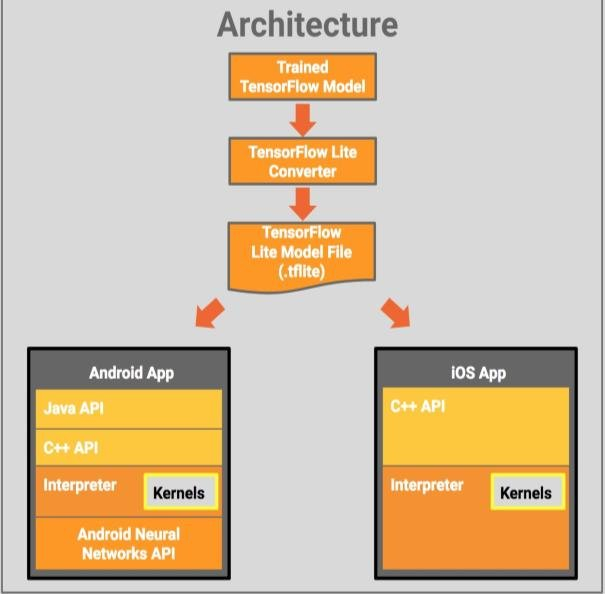
\includegraphics[width=0.5\linewidth]{fig/TFLite.jpg}
 	\caption{Implementatie flow van een getraind TensorFlow model naar de applicatie}
 	\label{fig:tflite}
\end{figure}

%anders formuleren
TensorFlow Lite is het antwoord van TensorFlow om CNN modellen te optimaliseren voor mobiel gebruik (figuur: \ref{fig:tflite}).
TensorFlow Lite zorgt ervoor dat het model een lage latency heeft en een kleine binaire grootte.
Het converteren kan makkelijk worden uitgevoerd via de volgende lijnen code in Python.

\begin{lstlisting}[language=Python, caption=Converteren van TensorFlow naar een TensorFlow Lite model]
import tensorflow as tf

converter = tf.lite.TFLiteConverter.from_saved_model(saved_model_dir)
tflite_model = converter.convert()
\end{lstlisting}	

Het TensorFlow Lite framework geeft ook de mogelijkheid om verdere optimalisaties zoals pruning en quantisatie uit te voeren na het converteren.
Het TensorFlow Lite model is ook compatibel met android en IOS.
Bij Android kan TensorFlow gebruik maken van de Neural Network API (NNAPI) ... die beschikbaar is vanaf Android 8.1.
Deze API kan gebruikt worden om netwerk modellen te versnellen met de GPU, DSP en NPU.

\subsection{PyTorch Mobile}
\begin{figure}[!ht]
    \centering
 	\includegraphics[width=0.5\linewidth]{fig/PyTorch-mobile.png}
 	\caption{Implementatie flow van een getraind PyTorch model naar de applicatie met code}
 	\label{fig:pt_mobile}
\end{figure}

PyTorch biedt zoals TensorFlow ook de mogelijk om het model te optimaliseren naar PyTorch Mobile.
In figuur: \ref{fig:pt_mobile} is te zien welke lijnen code er moeten worden uitgevoerd om een PyTorch model te converteren naar een PyTorch mobile model.
PyTorch mobile zit nog in zijn beta fase, dus hierbij kunnen er onverwachte complicaties optreden.
Een ander framework is Caffe2 dit framework focust ook op mobiele implementaties, maar het framework is ondertussen ge\"intrigeerd met PyTorch.
Ook is het PyTorch framework compatibel met android en IOS.
%meer over caffe


%TVM en qualcom

In de paper geschreven door \cite{luo_comparison_2020} wordt PyTorch Mobile vergeleken met Tenserfolow Lite voor verschillende netwerk architecturen en een model getraind met dezelfde data.
Voor alle netwerk architecturen in deze paper geeft de optimalisatie naar TensorFlow Lite de kleinste bestand grootte van het model. 
Uit deze paper is ook af te leiden dat de optimalisatie naar een mobiel model niet alleen afhankelijk is van het framework maar ook van de netwerk architectuur.
Zo geeft TensorFlow Lite volgens \cite{luo_comparison_2020} betere latency resultaten voor de zwaardere netwerken (ResNet50, InceptionV3, DenseNet121) dan PyTorch Mobile.
Maar PyTorch Mobile heeft op zijn beurt wel een betere latency voor SqueezeNet en MobileNetV2.
Dus uit deze paper kunnen we afleiden dat TensorFlow Lite het beste de bestands grootte verkleint, maar dat de netwerk architectuur ook een rol speelt.

\cite{febvay_low-level_2020} vergelijkt TensorFlow Lite met MACE voor verschillende neurale netwerken (SqueezeNet, MobileNetV1/V2).
Hierbij geeft TensorFlow Lite het beste resultaat, TensorFlow Lite gaf een Top-1 resultaat van 69,19\% en MACE gaf een top-1 resultaat van 66.84\% bij MobileNetV1.
Ook voor de latency gaf TensorFlow Lite in de meeste gevallen de beste resultaten buiten bij het gebruik van 4 of 6 CPU cores, dan gaf MACE betere resultaten.  

\section{Converteren naar framework voor mobiele implementatie}
Het doel van deze masterproef is om een bestaand netwerk op een mobiel platform te krijgen.
Dus zullen de object detectoren die ontworpen zijn met bovenstaande tools (Detectron2, MMDetection, ImagAI en Darkflow), geconverteerd moeten worden naar een framework voor mobiele implementatie.
Object detectoren zijn complexe systemen waarbij het converteren naar een ander framework complex of zelfs niet mogelijk zal worden.
In deze paragraaf zal per objectdetector bibliotheek gekeken worden wat de mogelijkheden zijn om van een detector model naar een mobiele implementatie te gaan.
De eerste stap zal zijn om te kijken welke mogelijkheden er zijn zonder te converteren naar een ander framework.
Een tweede stap is via Open Neural Network Exchange (ONNX) het huidige detectie model converteren naar een andere framework.
Een derde stap is verder zoeken naar een alternatief als de eerste twee methodes niet lukken.

%ONNX
\subsection{ONNX}
\cite{onnx_onnx_2017} biedt de mogelijkheid om verschillende tools/frameworks samen te laten werken.
Hierbij wordt een bestaand model geconverteerd naar een ONNX model, en dit model kan op zijn beurt geconverteerd worden naar het gewilde framework.
ONNX ondersteund niet elk machine learning framework, maar toch wel de meest bekende.
Het ONNX framework biedt zelf ook de mogelijkheid om een model te deployen en te optimaliseren voor mobiel gebruik.
ONNX dient goed als overkoepelend framework dat er voor zorgt dat verschillende frameworks compatibel zijn met elkaar.
Volgens de website zijn er 23 frameworks die naar het ONNX framework geconverteerd kunnen worden en een CNN kunnen ontwerpen en trainen. 
Om dan geconverteerd te worden naar een framework dat het model kan omzetten naar een mobile versie.
Een ander manieren om een model te gebruiken over verschillende frameworks in plaats van ONNX hangt af van de compatibiliteit tussen frameworks.
Bepaalde frameworks zullen zelf een methode hebben om modellen van andere frameworks in te laden.

\subsection{Van MMDetection naar detectie model voor mobile implementatie}
%MMDetection
Voor het testen van MMDetection nemen we de Kitty dataset ... waarmee we een detector trainen via transfer learning, hiervoor gebruiken we de Mask-rcnn detector.
Vermits MMDetection bovenop PyTorch werkt gaan we eerst proberen om met PyTorch Mobile te werken, dit gaat via de volgende lijnen code.

\begin{lstlisting}[language=Python, caption=Converteren van MMDetection naar een PyTorch Mobile]
import torch
import torchvision
from torch.utils.mobile_optimizer import optimize_for_mobile

model.eval()
example = torch.rand(1, 3, 224, 224)
traced_script_module = torch.jit.trace(model, example)
traced_script_module_optimized = optimize_for_mobile(traced_script_module)
traced_script_module_optimized._save_for_lite_interpreter("model.ptl")
\end{lstlisting}

Voordat het model kan geoptimaliseerd worden moet het python afhankelijk model worden omgezet in TorchScript. 
Deze TorchScript module kan dan verder geoptimaliseerd worden voor mobiel gebruik.
Het omzetten naar de scriptmodule geeft een TypeError fout waardoor het optimaliseren voor mobiel niet lukt.

Een andere manier om naar een mobiele implementatie te gaan is door het model eerst om te zetten naar het .onnx formaat.
MMDetection ondersteund de conversie naar ONNX, maar dit zit nog in zijn experimentele fase.
In de documentatie van MMDetection kan er een lijst gevonden worden met detectiemodellen die ondersteuning hebben voor het exporteren naar ONNX ... .
Ook heeft ONNX 'opsets' met daarin de operaties die ONNX ondersteund, niet elk framework past dezelfde opset versie toe wat later voor problemen kan zorgen.
Elke bibliotheek/framework moet dezelfde 'opset' implementeren anders zullen er operaties zijn die niet compatibel zijn met het gewilde framework voor mobiele implementatie.
Via de volgende lijn code is het mogelijk om het MMDetection model om te zetten naar een ONNX model.

\begin{lstlisting}[language=Python, caption=Converteren van MMDetection naar een onnx bestand]
!python ./tools/deployment/pytorch2onnx.py <config_file> <checkpiont_file> 
	--output-file <output file>
\end{lstlisting}

pytorch2onnx.py is het MMDetection script om een model te converteren naar ONNX formaat.
De config file is het bestand dat het neuraal netwerk beschrijft.
En de checkpoint file is een file die tijdens het trainen wordt aangemaakt als checkpoint.
Het finale model is vaak terug te vinden als latest.pth, dit is het laatste checkpoint dat na het trainen wordt aangemaakt.
Op het einde van deze lijn code is het mogelijk om nog extra opties toe te voegen die in de MMDetection documentatie ... terug te vinden zijn.
Bovenstaande lijn code converteert het MMDetection model succesvol naar een ONNX model.
Wel moet er bij vermeld worden dat dit MMDetection model een \'e\'envoudig model is waarbij geen speciale aanpassingen zijn gedaan.
Dus bij complexere modellen zou het resultaat anders kunnen zijn.

Het gegenereerde .onnx model is vervolgens geconverteerd naar een TensorFlow Lite model via de volgende lijnen code.

\begin{lstlisting}[language=Python, caption=Converteren van ONNX bestand naar een TensorFlow Lite model]
import tensorflow as tf
import onnx
from onnx_tf.backend import prepare
	
#ONNX model inladen 
onnx_model = onnx.load("model.onnx")  # inladen onnx model
output = prepare(onnx_model)
output.export_graph('tf_model.pb') # model exporteren naar TensorFlow model

#Ingeladen model omzetten naar TensorFlow Lite model
converter = tf.lite.TFLiteConverter.from_saved_model('tf_model.pb')
converter.target_spec.supported_ops = [
	tf.lite.OpsSet.TFLITE_BUILTINS, # enable TensorFlow Lite ops.
	tf.lite.OpsSet.SELECT_TF_OPS # enable TensorFlow ops.
]
tflite_model = converter.convert() # converteer model
\end{lstlisting}

Eerst moet het ONNX model ingeladen worden als een standaard TensorFlow model.
Vervolgens moest bij het converteren naar een TensorFlow Lite model eerst vermeld worden welke opsets er ondersteund moeten worden.
Het effectief converteren naar een TensorFlow Lite model duurt een hele tijd .... .

Om een model te converteren naar CoreML zijn er 3 mogelijkheden.
Eerst is rechtstreeks converteren vanuit PyTorch, daarvoor moeten we eerst ons model omzetten in een torchscript.
Maar dan stoot men op hetzelfde probleem als bij de PyTorch Mobile implementatie, waarbij het omzetten naar torchscript een TypeError geeft.
De tweede manier is via ONNX maar dat raad Apple af omdat dit in de volgende versie van CoreML niet meer ondersteund wordt, CoreML biedt ook maar ondersteuning tot en met opset versie 10.
Vanuit ONNX converteren gaat via de volgende lijnen code, maar vermits dit in later versies niet meer ondersteund wordt is deze methode niet uitgetest.

\begin{lstlisting}[language=Python, caption=Converteren van ONNX bestand naar een CoreML model]
import coremltools as ct

model  = ct.converters.onnx.convert(model='my_model.onnx')
\end{lstlisting}

De derde manier is rechtstreeks via TensorFlow convert, maar dit is een vrij omslachtige manier omdat we dan de volgende converties moeten maken MMDetection -> ONNX -> TensorFlow -> CoreML.
%heeft geen keras model wanneer het van tf komt.

%onnxruntime

%mace

\subsection{Van Detectron2 naar mobile implementatie}
%Detectron2

\subsection{Van ImageAI naar mobile implementatie}
%ImageAI

\subsection{Van DarkFlow naar mobile implementatie}
%DarkFlow


\section{Van een object herkening model naar een mobiele implementatie}

\section{Implementatie op mobiele platformen}
%meer tijd spenderen aan het vergelijken tussen verschillende frameworks, en hoe een bestaand model op een mobiel apparaat
%te krijgen
Uit paragraaf 3.1 kan er afgeleidt worden dat sommige frameworks ondersteuning bieden voor het optimaliseren van het machine learning model naar een lichtere versie.
Dus het bestaande CNN model zou naar \'e\'en van deze frameworks geconverteerd moeten worden zodat er gebruik gemaakt kan worden van de mobiele optimalisatie die dat framework ondersteund.
Niet elk framework zal even compatibel zijn met het bestaande model, er zal dus gekeken moeten worden tussen welke frameworks een conversie mogelijk is.
Ook zal niet elk framework de optimalisatie voor mobiele platformen op dezelfde manier toepassen.
Dus het converteren van het standaard model naar het mobiele model zal voor elk framework een ander resultaat geven.
In deze paragraaf zal er besproken worden welke frameworks er compatibel zijn met elkaar en welke frameworks het beste optimaliseren voor een mobile implementatie.

We hebben al gezien dat voor het converteren van een model niet veel lijnen code nodig zijn. 
Maar dit is enkel het geval als het model in het zelfde framework is ontworpen.
Als het model in een ander framework is ontworpen en getraind is de eerste stap van het process om het CNN model naar het gewilde framework te converteren.


\section{Optimalisaties van neurale netwerken voor snelheid en bestandgrootte}
In deze paragraaf wordt er onderzocht welke optimalisaties er kunnen worden toegepast om de accuraatheid, snelheid en gebruikt geheugen te verbeteren.
Maar het optimaliseren van een bepaalde factor zal vaak negatieve gevolgen hebben voor een andere factor, dit zal meestal de accuraatheid zijn.
Dus er zal een goede belans gevonden moeten worden tussen de optimalisatie en de negatieve gevolgen op de andere factoren.

%\subsection{Deep compression}
%De Deep compression methode voorgesteld door \cite{han_deep_2016} gebruikt 3 technieken om een model te verkleinen zodat het bruikbaar is op een mobiel apparaat.
%De 3 technieken zijn pruning, trained quantization en Huffman coding.
%Het doel van deze 3 technieken is om de opslag vereisten te verkleinen, met zo weinig mogelijk effect op de accuraatheid.

\subsection{Pruning}
Pruning is de eerste stap van de Deep comression methode voorgesteld door \cite{han_deep_2016}.
Bij het trainen van een CNN hebben bepaalde gewichten een grotere invloed op het resultaat.
Andere gewichten hebben weinig tot geen invloed op het resultaat.
Maar alle gewichten worden steeds berekend ongeacht hun invloed op het resultaat.
Bij pruning worden de gewichten met een kleine invloed op het resultaat verwijderd dit is weergegeven op figuur \ref{fig:pruning}. 
Waardoor er geen berekeningen meer moeten uitgevoerd worden voor de verwijderde gewichten.
Deze parameters moeten dan ook niet meer worden bijgehouden waardoor het CNN model minder geheugen in beslag neemt.
Eerst wordt het CNN op een normale manier getraind zonder pruning.
Vervolgens worden al de kleine gewichten onder een bepaalde treshold verwijderd.
volgens \cite{han_deep_2016} wordt voor VGG-16 het aantal parameters met factor 13 verminderd, voor AlexNet met een factor 9.
Deze methode heeft zeer weinig tot geen effect op de accuraatheid.
%connectie pruning, neuron pruning

\begin{figure}[!ht]
	\centering
	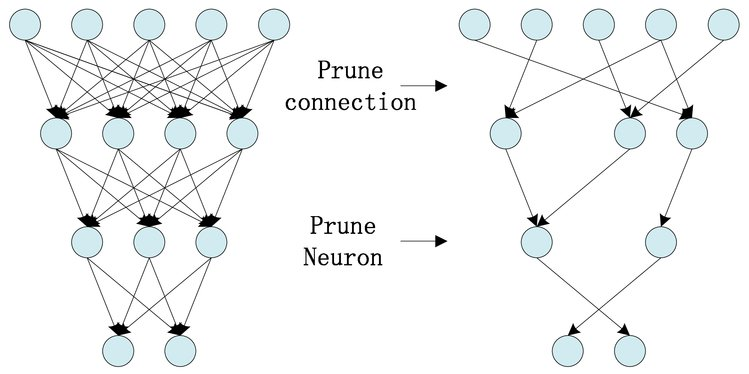
\includegraphics[width=0.65\linewidth]{fig/pruning.jpg}
	\caption{CNN voor en na pruning}
	\label{fig:pruning}
\end{figure}

\subsection{Parameter quantisatie}
Het quantiseren en delen van gewichten is een tweede methode voorgesteld door \cite{han_deep_2016}.
Een CNN bestaat uit miljoenen gewichten, en de waarde van elke van deze gewichten moeten op het systeem worden opgeslagen.
De default representatie van een waarde wordt opgeslagen als een floating point nummer wat 4 bytes in beslag neemt.
Dus voor miljoenen parameters hebben de gewichten veel schijfruimte nodig.
Een mogelijke oplossing hiervoor is quantiseren van gewichten, waarbij de getal representatie van de gewichten wordt verandert naar fixed point.
Hierbij worden de waarden van gewichten beperkt tot een set van beschikbare waardes.
Waarbij de waardes \"e\"enmalig worden opgeslagen en al de gewichten refereren naar een waarde van de vaste set met waardes.
Hoe kleiner de set met waardes is hoe minder geheugen er in beslag wordt genomen, maar een kleinere set van waardes zorgt ook voor een mindere accuratie.
Dus de grootte van de set moet goed worden gekozen zodat er niet te veel geheugen wordt gebruikt met een accepteerbare daling in accuratie.
\cite{han_deep_2016} past vervolgens Huffman encoding toe die een compressie uitvoert op de gekwantiseerde parameters.
%hashed net gebruikt hashes

\subsection{Convolutionele filter compressie}
een andere methode voorgesteld is Compressed Convolutional Filters.
Hierbij wordt de grootte van de kernel verkleind om het aantal parameters en rekenwerk te verminderen.
Maar door de kernels te verkleinen daalt de accuraatheid van het CNN.
%paper zoeken met weer uitleg

\subsection{Matrix factorisatie}
Hierbij worden grootte en complexe matrices opgesplitst in verschillende kleinere en simpelere matrices.

%\subsection{Vermijd fully connected lagen}
%Fully connected lagen zijn een basis component van neurale netwerken.
%Maar fully connected lagen genereren veel parameters, dus gebruiken ook veel geheugen.
%Ook voeren fully connected lagen veel berekening uit waardoor zij ook een vertragende factor zijn.
%Dus voor mobiele implementaties is het beter om geen of weinig fully connected lagen te gebruiken.

%\subsection{Wijzigen van de Kernel}
%Door met meer kernels te werken kan men meer informatie uit de data halen, maar dan worden er ook meer feature mappen gegenereerd.
%Deze feature mappen beschikken over veel informatie maar nemen meer geheugen in beslag.
%Een groter aantal feature mappen is meer data dus ook meer berekeningen en meer berekeningen maakt het systeem trager.
%Dus door het aantal kernels te verminderen worden er ook minder feature mappen gegenereerd.
%Dit zorgt voor een snelheids winst en meer vrij geheugen, maar er is dan wel een verlies aan informatie.

%De grootte van de kernel kan ook woorden aangepast zo kan men i.p.v. een 3x3 kernel met een 2x2 kernel werken.
%Door de kernelgrootte te verkleinen moeten er minder berekeningen worden uitgevoerd wat zorgt voor een snelheidswinst en meer vrij geheugen.
%Maar de door de kernelgrootte te verkleinen is er terug een verlies aan informatie.

%stride

%\subsection{Pooling laag optimalisatie}
%De pooling laag zorgt voor een vermindering in de dimensie van de feature map.
%deze vermindering van dimensie zorgt ervoor dat er minder parameters zijn, maar minder parameters betekent ook verlies aan informatie.
%Dus door wijzigingen aan te brengen aan de pooling laag kan de hoeveelheid data en rekenwerk verbeterd worden.

%De pooling laag kan naar voor worden geschoven in het CNN waardoor de dimensie van de feature map sneller kleiner wordt.
%Dit heeft als gevolg dat er met minder parameters verdergegaan moet worden, waardoor het model sneller wordt.
%Maar dit zorgt er ook voor dat bepaalde informatie sneller verloren gaat wat zorgt voor een lagere accuratie.
%Een andere vorm van pooling optimalisatie is gewoonweg meer pooling lagen toevoegen waardoor de dimensie van de feature mappen vaker verkleint wordt.
%Maar dit heeft ook een negatieve invloed op de accuraatheid.
%kernel vergroten

% \section{CNN architecturen voor mobiele platformen}
% Dit deel gaat over CNN architecturen die specifiek ontworpen zijn voor mobiele en embedded toestellen.
% Deze netwerk architecturen streven naar zo weinig mogelijk parameters en een zo snel mogelijke uitvoering zonder een te groot effect op de accuraatheid te hebben.
% Het overlopen van deze netwerken voor de masterproef is iets minder relevant vermits we een reeds getraind CNN willen optimaliseren.
% Dus dat netwerk is reeds getraind, maar er kan wel gekeken worden welke technieken deze architecturen gebruiken zodat het model gebruikt kan worden op een mobiel platform.

% \subsection{MobileNet}
% MobileNet is voornamelijk opgebouwd uit diepe afzonderlijke convoluties(depthwise separable convolution), om het aantal berekeningen te verminderen.
% Deze convoluties bestaan uit een depthwise convolutie, waarbij \'e\'en filter over elk input kanaal gaat waardoor er afzonderlijke feature maps onstaan.
% Vervolgens gebeurt er een pointwise convolutie die met een 1x1 convolutie de outputs samenvoegt.
% Deze manier van werken zorgt voor een grootte vermindering in het aantal parameters met een klein effect op de accuraatheid.
% VGG-16 heeft 138 miljoen parameters en een accuraatheid van 71.5\%, MobileNet heeft 4.2 miljoen parameters met een accuraatheid van 70.6\%.
% Ondertussen is er al een MobileNetV2 ... en ook een MobileNetV3 ... .

% \subsection{EfficientNet}


% \subsection{TinyYOLO}

%%%%%%%%%%%%%%%%%%%%%%%%%%%%%%%%%%%%%%%%%%%%%%%%%%%%%%%%%%%%%%%%%%%% 
%                                                                 %
%                            CHAPTER                              %
%                                                                 %
%%%%%%%%%%%%%%%%%%%%%%%%%%%%%%%%%%%%%%%%%%%%%%%%%%%%%%%%%%%%%%%%%%% 
%\chapter{Richtlijnen voor formules}
%%%%%%%%%%%%%%%%%%%%%%%%%%%%%%%%%%%%%%%%%%%%%%%%%%%%%%%%%%%%%%%%%%%% 
%                                                                 %
%                            CHAPTER                              %
%                                                                 %
%%%%%%%%%%%%%%%%%%%%%%%%%%%%%%%%%%%%%%%%%%%%%%%%%%%%%%%%%%%%%%%%%%% 
\chapter{Planning}
\section{Herwerkte planning \ref{fig:plan}}
\begin{figure}[!ht]
	\centering
	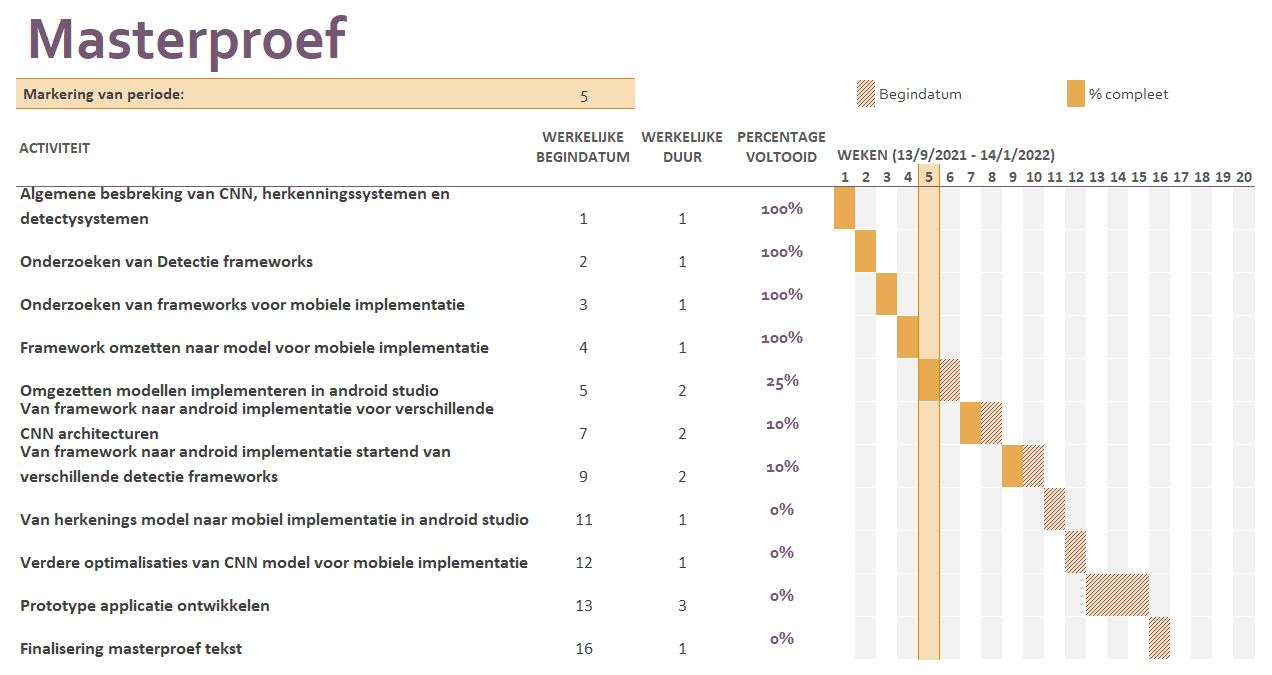
\includegraphics[width=1.0\linewidth]{fig/planning.jpg}
	\caption{herwerkte planning.}
	\label{fig:plan}
\end{figure}
\chapter{Compatibiliteit van herkenningssystemen}
Voor het herkenningssysteem bestuderen we de implementatie van de ResNet50 architectuur die in paragraaf \ref{resnet} werd besproken.
We vertrekken van een bestaand model dat voorgetraind is met het TensorFlow of het PyTorch framework om de verschillende mogelijkheden voor een mobiele implementatie te bestuderen.
Hierbij maken we gebruik van Google Colaboratory in CPU runtime om de modellen in te laden en te converteren.
Om het geconverteerd model te implementeren op een mobiel toestel maken we gebruik van Android Studio.
De ge\"implementeerde code is terug te vinden in de volgende github repository: \url{https://github.com/ThijsVercammen/Masterproef.git}.

% \section{ResNet50}
% \cite{he2015deep} heeft vastgesteld dat als het aantal lagen van een CNN toeneemt dat op een bepaald moment de training accuraatheid daalt.
% Dit verschijnsel noemt men de vanishing gradient.
% In paragraaf \ref{train} hebben we besproken hoe we de gradient kunnen berekenden tijdens het trainen van een CNN.
% Voor elke laag in het CNN moet de gradient opnieuw berekend worden door telkens opnieuw de afgeleide te berekenen.
% Hierdoor wordt de gradient steeds kleiner en kleiner tot deze een minimum bereikt.
% Waardoor de gewichten in de eerste lagen heel traag aanpassen of zelfs niet meer veranderen.
% \cite{he2015deep} die dit probleem hebben vastgesteld hebben dit opgelost door gebruik te maken van skip connections.
% Hierbij wordt de input van een laag rechtstreeks met een volgende laag die x aantal lagen verder ligt.
% Op deze manier worden de gradienten per laag niet meer kleiner.
% ResNet50 bestaat uit 50 convolutie lagen waarbij er een skip connection plaatsvindt per 3 lagen.
% De resnet50 architectuur is opgebouwd uit ResNet blokken die bestaan uit 3 convolutie lagen en 1 skip connection.

%https://github.com/tensorflow/models/blob/master/official/vision/image_classification/resnet/resnet_model.py
%https://github.com/priya-dwivedi/Deep-Learning/blob/master/resnet_keras/Residual_Networks_yourself.ipynb

\section{Van TensorFlow naar mobiel framework}
Voor het experiment van ResNet50 maken gebruiken we het standaard ResNet50 netwerk dat in TensorFlow ge\"implementeerd kan worden vanuit Keras.
Dit ResNet50 model is voorgetrained op de ImageNet dataset \cite{deng_2009_imagenet}. 
Dit netwerk kunnen we vervolgens hertrainen naar een gewenste functionaliteit.
Voor deze implementatie zullen we echter vertrekken van het ResNet50 Keras model dat reeds bestaat.

\subsection{TensorFlow Lite implementatie} \label{tf_h_conv}
Het inladen en converteren van het Keras model kan eenvoudig via de volgende Python code.

\begin{python}
model = tf.keras.applications.resnet50.ResNet50() # model inladen
converter = tf.lite.TFLiteConverter.from_keras_model(model) # init converter
tflite_model = converter.convert() # model converteren
open('model.tflite', 'wb').write(tflite_model) # model opslaan
\end{python}

Het ResNet50 model kan zonder problemen of aanpassingen rechtstreeks worden geconverteerd naar TFlite.
We vertrekken van een bestaand model dat voorgetraind is met het TensorFlow of het PyTorch framework om de verschillende mogelijkheden voor een mobiele implementatie te bestuderen.
In de tabel kunnen we zien welke TensorFlow operaties worden ondersteund door een TFLite equivalent.
Verder is in de tabel weergegeven welke TensorFlow operaties worden ondersteund door een TFLite equivalent en op welke operaties optimalisaties worden uitgevoerd tijdens het converteren. 
Bij deze optimalisaties worden operaties samengevoegd, verwijderd of vervangen door een constante.
Figuur \ref{fig:class_opt} laat zien welke optimalisaties er worden uitgevoerd op een ResNet50 convolutieblok.

\begin{figure}[!ht]
	\centering
	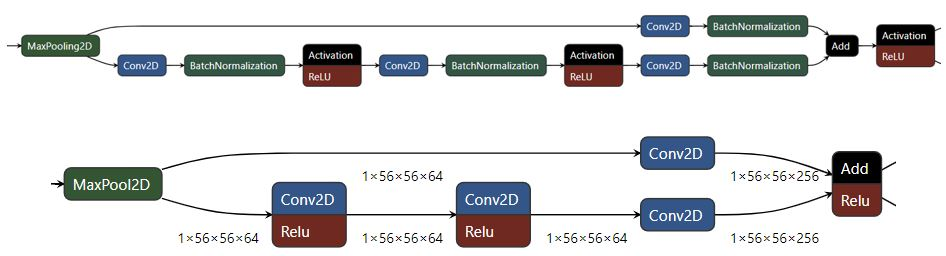
\includegraphics[width=1.0\linewidth]{fig/class_opt.jpg}
	\caption{ResNet50 convolutieblok voor en na TFLite conversie. BatchNorm en ReLu zijn hierbij samengevoegd met de Conv2D opperaties.}
	\label{fig:class_opt}
\end{figure}

Voor de android implementatie kunnen we metadata aan het model toevoegen.
Dit is niet noodzakelijk, maar vereenvoudigd de Android implementatie.
\begin{python} 
ImageClassifierWriter = image_classifier.MetadataWriter
model_p = "./model.tflite" # TFLite model
label_p = "./labels.txt" # label file voor label formaat
save_p = "./model_meta.tflite" # opslaan pad
input_norm_mean = 0.0
input_norm_std = 1.0
    
# metadata scrijver
writer = ImageClassifierWriter.create_for_inference(
    writer_utils.load_file(model_p), [input_norm_mean], [input_norm_std],
    [label_p])
    
# Voeg metadata aan het model toe en sla op
writer_utils.save_file(writer.populate(), save_p)
\end{python}

Omdat we deze metadata hebben toegevoegd heeft Android studio toegang tot al de relevante input en output informatie.
Vermits Android studio toegang heeft tot deze informatie kan het zelf code genereren om het TFLite model te implementeren.
De code die gegenereerd wordt is implementeerbaar in Java en Kotlin.
Onderstaande Java code heeft Android studio voor ons gegenereerd.
Het enige wat nu nog rest is een afbeelding inlezen als bitmap en de output afhandelen.
\newpage

\begin{python}
Model model = Model.newInstance(context);

// Creates inputs for reference.
TensorImage image = TensorImage.fromBitmap(bitmap);

// Runs model inference and gets result.
Model.Outputs outputs = model.process(image);
List<Category> probability = outputs.getProbabilityAsCategoryList();

// Releases model resources if no longer used.
model.close();
\end{python}

\begin{table}[!ht]
    \caption{Alle operaties die terug te vinden zijn in het TensorFlow ResNet50 model en hun compatibiliteit met andere frameworks}
\begin{tabular}{ccc}
    \hline
    TensorFlow Operaties & TensorFlow \textrightarrow TFLite & ONNX Opset \\
    \hline
    AddV2 & Ondersteund & 1 \\
    BiasAdd & Samengevoegd & 1 \\
    %Const & constant & 1 \\
    Conv2D & Ondersteund & 1 \\
    FusedBatchNormV3 & Samengevoegd & 6 \\
    Identity & Verwijderd & 1 \\
    MatMul & Ondersteund & 1 \\
    MaxPool & Ondersteund & 1 \\
    Mean & Ondersteund & 1 \\
    NoOp & Verwijderd & / \\
    %Pack & Ondersteund & 1 \\
    Pad & Ondersteund & 1 \\
    Placeholder & Constant & 1 \\
    Relu & Samengevoegd & 1 \\
    Softmax & Ondersteund & 1 \\
    %StatefulPartitionedCall & Ondersteund & / \\
    \hline
\end{tabular}
\label{tab:TFop}
\end{table}

\subsection{ONNX implementatie} \label{classonnx}
Het TensorFlow model kunnen we converteren naar ONNX met tf2onnx bibliotheek.
De tf2onnx bibliotheek ondersteunt TensorFlow en TFLite.
Hierdoor kunnen we beide modellen converteren naar ONNX.
In tabel \ref{tab:TFop} kunnen we afleiden welke operaties ondersteund zijn door ONNX en vanaf welke opset versie deze operaties worden ondersteund.
De minimale opset moet versie 6 zijn vanwege de FusedBatchNormV3 operatie die pas vanaf versie 6 wordt ondersteund.
Via het volgende CLI commando kunnen we het TensorFlow model converteren naar ONNX of kunnen we het TFLite model converteren naar ONNX door de optie --tflite mee te geven.

\begin{python}
python -m tf2onnx.convert --saved-model ./model --output model.onnx
\end{python}

Voor de Android implementatie van het ONNX model maken we gebruik van Kotlin in plaats van Java.
De voornaamste reden hiervoor is dat de Onnxruntime documentatie Kotlin code gebruikt voor de Java API.
%voorbeelden ook in Kotlin zijn ge\"implementeerd.
Via onderstaande Kotlin code kan het ONNX model worden uitgevoerd in Android studio.

\begin{python} 
var env = OrtEnvironment.getEnvironment()
// lees het ONNX model als byteArray
var session = env.createSession(resources.openRawResource(R.raw.model_tf).readBytes())
// Maak een input tensor aan
var input_tensor = OnnxTensor.createTensor(env, imgData, shape)
// maak een inputmap aan
var inputs = Collections.singletonMap("input_1", t1)
// voer model uit
val output = session?.run(inputs)
\end{python}

We lezen het ONNX model in als een byteArray.
Dit ONNX model hebben we opgeslagen in de res/raw folder van het Android studio project.
Vervolgens wordt er een ONNX input tensor aangemaakt.
Hierbij wordt de data van de afbeelding als FloatArray meegegeven net als de vorm van de input tensor die het ONNX model verwacht.
Het ONNX model verwacht een input vorm [1, hoogte, breedte, 3] deze vorm is van het NHWC formaat eerder besproken in \ref{nhwc}.
Voordat we het model kunnen uitvoeren moeten we de input tensor aan een map toevoegen.
De keys van deze map zijn de namen van de inputs die het ONNX model verwacht, de values van de map zijn de input tensoren.
De input namen zijn terug te vinden in de output boodschappen van tf2onnx converter.
%We moeten er wel bij vermelden dat TFLite enkel variabelen van het type float32 en int8 ondersteund.
%De tf2onnx converter maakt standaard gebruik van ONNX opset versie 9.
%Bij het converterent van TensorFlow naar ONNX onder standaard omstandigheden krijgen we de volgende fout 
%\textcolor{red}{ValueError: StridedSlice: only strides=1 is supported}.  
%Voor het converteren van TensorFlow naar ONNX is minstens opset versie 10 nodig.

\section{Van PyTorch naar mobiele implementatie}
Voor de PyTorch implementatie gebruiken we van het ResNet50 model uit de Torchvision bibliotheek.
Dit model is voorgetraind op de ImageNet dataset (\cite{deng_2009_imagenet}) .
Dit netwerk kunnen we vervolgens hertrainen voor een gewenste functionaliteit.
Voor deze implementatie zullen we echter vertrekken van het reeds bestaande ResNet50 Torchvision model.

\subsection{PyTorch Mobile implementatie} \label{py_class}
Via de volgende Python code kunnen we een ResNet50 Torchvision model inladen en converteren voor mobiel gebruik.

\begin{python}
model = models.resnet50(pretrained=True) # model inladen
model.eval() # model in uitvoer modus
example = torch.rand(1, 3, 224, 224) # voorbeeld input
# Torchscript module genereren
traced_script_module = torch.jit.trace(model, example) 
# optimalisaties voor mobiel gebruik uitvoeren op de scriptmodule
traced_script_module_optimized = optimize_for_mobile(traced_script_module)
# model opslaan voor mobiel gebruik
traced_script_module_optimized._save_for_lite_interpreter("./model.pt") 
\end{python}

Het ResNet50 model wordt zonder problemen geconverteerd, geoptimaliseerd en opgeslagen voor mobiel gebruik.
In tabel \ref{tab:PYop} zien we welke operaties er terug te vinden zijn in het Torchvision model en wat er met deze operaties gebeurt tijdens de conversie.
Het mobiel model kunnen we vervolgens implementeren in Android studio.

\begin{table}[!ht]
    \caption{Alle operaties die terug te vinden zijn in het Torchvision ResNet50 model en hun compatibiliteit met andere frameworks}
\begin{tabular}{ccc}
    \hline
    TorchScript & TorchScript \textrightarrow  ge\"optimaliseerd torchscript & ONNX Opset \\
    \hline
    Add & Ondersteund & 1 \\
    AdaptiveAvgPool2d & Ondersteund & 1 \\
    BatchNorm2d & Samengevoegd & 1 \\
    Conv2d & Ondersteund & 1 \\
    Flatten & Ondersteund & 1 \\
    Linear & Ondersteund & 1 \\
    MaxPool2d & Ondersteund & 1 \\
    ReLu & Samengevoegd & 1 \\
    \hline
\end{tabular}
\label{tab:PYop}
\end{table}

Het ResNet50 Torchvision model verwacht een genormaliseerde input dat standaard is voor elk Torchvision model.
Door de input te normaliseren verwacht het model altijd een pixelwaarde met een gemiddelde van 0 en een standaarddeviatie van 1.

\begin{equation}
    \begin{aligned}
	\textrm{TORCHVISION\_NORM\_MEAN\_RGB}  = \{0.485, 0.456, 0.406\} \\
	\textrm{TORCHVISION\_NORM\_STD\_RGB}  = \{0.229, 0.224, 0.225\}
    \end{aligned}
\end{equation}

Het model kan vervolgens met de volgende Java code eenvoudig ge\"implementeerd worden in Android studio. 

\begin{python}
module = Module.load(assetFilePath(MainActivity.this, "model.ptl"));
Tensor inputTensor = TensorImageUtils.bitmapToFloat32Tensor(bitmap,
            TensorImageUtils.TORCHVISION_NORM_MEAN_RGB, 
            TensorImageUtils.TORCHVISION_NORM_STD_RGB);
Tensor outputTensor = module.forward(IValue.from(inputTensor)).toTensor();
\end{python}

\subsection{ONNX implementatie} \label{py_onnx}
Het ResNet50 Torchvision model kunnen we in Python eenvoudig converteren naar ONNX via de volgende code:

\begin{python}
torch.onnx.export(model, # model 
    example,             # model input
    "model_py.onnx",     # waar opslaan
    input_names = ['input_1'], # input namen
    output_names = ['output']) # output namen    
\end{python}

Het gegenereerde ONNX model kan ge\"implementeerd worden in Android studio.
Het ONNX model verwacht een input vorm [1, 3, hoogte, breedte], deze vorm is van het NCHW formaat eerder besproken in \ref{nhwc}.
Het geconverteerd PyTorch model verwacht een genormaliseerde input van een afbeelding.
De genormaliseerde waarde kan via de volgende formule berekend worden.

\begin{equation}
    \begin{aligned}
	\textrm{genormaliseerd}  = \frac{(\textrm{waarde} - \textrm{mean})}{\textrm{std}} \\
    \textrm{mean}  = \{0.485, 0.456, 0.406\} \\
	\textrm{std}  = \{0.229, 0.224, 0.225\}
\end{aligned}
\end{equation}

In deze formule is mean de gemiddelde waarde en std de standaarddeviatie waarmee Torchvision een normalisatie uitvoert.
De mean en std bevatten drie waarde.
Dit is omdat bij Torchvision elk kleurkanaal zijn eigen mean en std waarde heeft voor normalisatie.
De rest van de implementatie in Android studio is identiek aan de ONNX implementatie van het TensorFlow model zoals besproken in \ref{classonnx}. 

\section{Samenvatting}
We hebben gezien dat herkenningssystemen volledig ondersteund zijn.
De modellen van het PyTorch en TensorFlow framework worden zonder problemen geconverteerd naar een model voor mobiel gebruik.

Voor het TensorFlow model kunnen we in Python ons model converteren met de onderstaande code.
Dit model is implementeerbaar in Android studio.
TensorFlow geeft ons de mogelijkheid om hier Metadata aan toe te voegen, waardoor Android studio de nodige code voor ons genereert.

\begin{python}
    converter = tf.lite.TFLiteConverter.from_keras_model(model)
    tflite_model = converter.convert()
    open('model.tflite', 'wb').write(tflite_model) # model opslaan
\end{python}

Het PyTorch model kunnen we ook eenvoudig converteren met onderstaande Python code.
We moeten wel rekening houden met het feit dat het Torchvision model een genormaliseerde input verwacht.

\begin{python}
model.eval() # model in uitvoer modus
example = torch.rand(1, 3, 224, 224) # voorbeeld input
traced_script_module = torch.jit.trace(model, example) 
traced_script_module_optimized = optimize_for_mobile(traced_script_module)
traced_script_module_optimized._save_for_lite_interpreter("./model.pt") 
\end{python}

Het TensorFlow model kan naar ONNX geconverteerd worden via het volgende CLI-commando.

\begin{python}
python -m tf2onnx.convert --saved-model ./model --output model.onnx
\end{python}

Voor PyTorch gebeurt de conversie naar ONNX via onderstaande Python code.

\begin{python}
torch.onnx.export(model, example, "model.onnx",
        input_names = ['input'], output_names = ['output'])    
\end{python}

De twee ONNX modellen worden op dezelfde ge\"implementeerd in Android studio.
Hierbij moeten we wel rekening houden met het input formaat.
Het PyTorch ONNX model verwacht NCHW formaat en het TensorFlow ONNX model verwacht NHWC formaat.
Bovendien verwacht het PyTorch ONNX model een genormaliseerde input en het TensorFlow ONNX model geen genormaliseerde input.
\chapter{Compatibiliteit van detectie systemen}
Voor detectiesystemen bestuderen we uitgebreid de mobiele implementatie van de Faster-RCNN architectuur met een ResNet50 backbone en de YOLO architectuur.
Voor deze modellen vertrekken we vanuit het PyTorch en TensorFlow framework om vervolgens de mogelijke paden te bestuderen naar een mobiele implementatie.
Hierbij maken we gebruik van Google Colaboratory met een CPU runtime om de modellen in te laden en te converteren.
Om het geconverteerde model te implementeren op een mobiel toestel gebruiken we Android Studio.
De volledige ge\"implementeerde code is terug te vinden in de volgende github repository: \url{https://github.com/ThijsVercammen/Masterproef.git}.

\section{Faster-RCNN naar mobiel mobiele implementatie}
Het Faster-RCNN model waarmee we starten is terug te vinden in de TensorFlow object detection API.
Dit Faster-RCNN model is voorgetraind met de COCO 2017 dataset (\cite{lin2015microsoft}) en maakt gebruik van een ResNet50 backbone.
We gaan dit model converteren naar een ONNX en TFLite formaat zodat dit model ge\"implementeerd kan worden in Android studio.
Vervolgens vertrekken we vanuit PyTorch waar we het Faster-RCNN model kunnen terugvinden in de Torchvision bibliotheek.
Dit model is ook een Faster-RCNN model dat voorgetraind is op de COCO 2017 dataset.
Vervolgens converteren we het Torchvision model naar een ONNX of PyTorch mobile formaat dat we kunnen implementeren in Android studio.

\subsection{Van TensorFlow naar TFLite implementatie} \label{rcnn_tf}
Het Faster-RCNN model van de TensorFlow object detection API is terug te vinden in de TensorFlow Hub.
Dit model kan eenvoudig worden ingeladen met de volgende Python code.

\begin{python}
import tensorflow_hub as hub
hub_model = hub.load("https://tfhub.dev/tensorflow/faster_rcnn/resnet50_v1_640x640/1")
\end{python}

De TensorFlow object detection API stelt zelf een manier voor om een model te converteren naar het TFLite formaat.
Hierbij wordt via een script (export\_tflite\_graph\_tf2.py) een model gegenereerd dat geoptimaliseerd is voor TFLite conversie.
Op deze manier zou de rest van de conversie gelijkaardig moeten zijn aan de conversie van het ResNet50 netwerk besproken in \ref{tf_h_conv}.
Maar de TensorFlow object detection API ondersteund enkel de TFLite conversie voor de SSD en Centernet architecturen.
Als we het script toch proberen uit te voeren dan krijgen we de volgende error: 
\textcolor{red}{ValueError: Only ssd or center\_net models are supported in tflite. Found faster\_rcnn in config.}

Als we het model willen converteren zonder gebruik te maken van het optimalisatie script zullen we standaard TensorFlow operaties aan het TFLite model moeten toevoegen.
Deze operaties moeten worden toegevoegd omdat we de ConcatV2 operatie niet kunnen converteren naar de TFLite concatenation operatie.
% waarom?????????????????????????????????????????
Om dit te realiseren moet de TensorFlow core bibliotheek worden toegevoegd aan Android studio zodat alle operaties uitgevoerd kunnen worden.

\begin{python}
converter = tf.lite.TFLiteConverter.from_keras_model(hub_model) # init converter
converter.target_spec.supported_ops = [
    tf.lite.OpsSet.TFLITE_BUILTINS, # enable TensorFlow Lite ops.
    tf.lite.OpsSet.SELECT_TF_OPS # enable TensorFlow ops.
]
tflite_model = converter.convert() # converteer
open('model.tflite', 'wb').write(tflite_model) # model opslaan
\end{python}

Na het uitvoeren van bovenstaande Python code hebben we een TFLite model dat een input verwacht van de vorm [1,1,1,3].
Om dit TFLite model te kunnen uitvoeren moeten we de grootte van de inputafbeelding naar een hoogte en een breedte van 1 veranderen.
Een input die bestaat uit 1 pixel zou nooit voldoende informatie bevatten om objecten in de originele afbeelding te gaan detecteren.

Om dit probleem op te lossen defini\"eren we het model van de TensorFlow object detection API als een Keras laag.
Op deze manier kunnen we de input specifi\"eren en extra lagen gaan toevoegen via onderstaande Python code.

\begin{python} \label{testref}
layer = hub.KerasLayer(hub_model) # definieer als Keras laag
inputs = tf.keras.Input(shape=[416,416,3], dtype=tf.uint8) # specifieer input
x = layer(x) # genereer een output
output = [x["detection_classes"], x["detection_boxes"], x["detection_scores"], x["num_detections"]]
model = tf.keras.Model(inputs, output) # groepeer lagen tot model
\end{python}

Het formaat van de input kunnen we kiezen.
Een groot formaat geeft een beter resultaat, maar bevat meer data dus er moeten meer berekeningen worden uitgevoerd.
Een klein formaat geeft een minder goed resultaat, maar is sneller omdat er minder berekeningen uitgevoerd moeten worden.
Het datatype van de input moet uint8 zijn omdat het ingeladen model dit datatype verwacht.
Een ander voordeel van dit model is dat ConcatV2 operaties zonder problemen kunnen omgezet worden in de TFLite concatenation operatie.

De TFLiteConverter zal de namen van de verschillende outputs van het Faster-RCNN model veranderen.
Tijdens de conversie zal de volgorde van de vier outputs willekeurig veranderd worden.
De 4 outputs die wij zullen gebruiken in de Android studio implementatie zijn:

\begin{itemize}
	\item detection\_classes \textrightarrow StatefulPartitionedCall:0
	\item detection\_boxes \textrightarrow StatefulPartitionedCall:1
	\item detection\_scores \textrightarrow StatefulPartitionedCall:2
    \item num\_detections \textrightarrow StatefulPartitionedCall:3
\end{itemize}

%Voor een object detectie model te converteren kan er ook gebruik gemaakt worden van de standaard TFLiteConverter.
%Bij het converteren naar TFLite kan de ConcatV2 opperatie niet geconverteerd worden naar de TFLite concatenation opperatie.
%in het huidig model zijn er 2 gevallen waarbij de tf.ConcatV2 niet wordt geconverteerd naar tfl.concatenation.
%wat deze 2 gevallen van tf.ConcatV2 gemeenschappelijk hebben is dat zij een input krijgen van de tfl.div opperatie die is geconverteerd van tf.Realdiv.
%Door het toevoegen van TensorFlow Flex opperaties kan het model zonder problemen geconverteerd worden naar een TFLite model.
%Omdat we gebruik maken van Flex opperaties moet de TensorFlow core bibliotheek mee ge\"implementeerd worden in Android studio.
In tabel \ref{tab:TF_det_op} zien we wat er gebeurt met de operaties van het Faster-RCNN model tijdens de conversie naar TFLite.
Uiteraard komen de operaties van het ResNet50 model eerder besproken in (\ref{tab:TFop}) ook voor in het Faster-RCNN.
Deze operaties zullen op dezelfde manier geconverteerd worden naar TFLite.

Om Android studio zelf de code te laten genereren zoals bij het herkenningssysteem moeten we Metadata aan het model toevoegen. 
Bij het toevoegen van Metadata aan het TFLite model krijgen we de volgende fout: \textcolor{red}{Keyerror 2708.}
Deze fout geeft weinig informatie, maar de oorzaak is dat de methode die de Metadata aan het model toevoegt maximaal 4 outputs verwacht.
Het geconverteerd Faster-RCNN model heeft echter 8 outputs.
Door het aantal outputs te reduceren tot 4 outputs kunnen we Metadata succesvol aan het model toevoegen. % \ref{testref}.
Het uitvoeren van het model met Metadata in Android studio geeft de volgende error: 
\textcolor{red}{java.lang.IllegalArgumentException: Cannot copy from a TensorFlowLite tensor (StatefulPartitionedCall:2) with 1200 bytes to a Java Buffer with 4 bytes.}
\newline
Deze fout onstaat doordat tijdens het converteren naar TFLite de output informatie is gewijzigd.
De converter wijzigt namelijk de grootte van de output arrays naar 1, terwijl er meerdere resultaten worden geproduceerd.
Bijvoorbeeld de output van de detection\_boxes is [1, 300, 4], maar volgens de metadata is de output grootte [1, 1, 1] voor de bounding box co\"ordinaten.
Android studio genereert volgens de metadata een output buffer met grootte [1, 1, 1] die veel te klein is.

Om de grootte van de output buffers zelf te defini\"eren kunnen we gebruik maken van de TensorFlow Lite Interpreter API.
Via onderstaande Java code kunnen we het TFLite model uitvoeren in Android studio door gebruik te maken van de TensorFlow Lite Interpreter API

\begin{python}
Interpreter.Options tfliteOptions = new Interpreter.Options();
Interpreter tflite = new Interpreter(loadModelFile(), tfliteOptions);
tflite.runForMultipleInputsOutputs(inputs, outputs);

private MappedByteBuffer loadModelFile() throws IOException {
    AssetFileDescriptor fileDescriptor = this.getAssets().openFd("model.tflite");
    FileInputStream inputStream = new FileInputStream(fileDescriptor.getFileDescriptor());
    FileChannel fileChannel = inputStream.getChannel();
    long startOffset = fileDescriptor.getStartOffset();
    long declaredLength = fileDescriptor.getDeclaredLength();
    return fileChannel.map(FileChannel.MapMode.READ_ONLY, startOffset, declaredLength);
}
\end{python}

Hierbij kunnen we het TFLite model implementeren zonder er metadata aan toe te voegen.
De vereiste informatie om de correcte buffers te defini\"eren kan uit het niet geconverteerde model gehaald worden.
Het TFLite model bevat de juiste informatie voor de inputbuffer.
via deze informatie kan de juiste inputbuffer worden aangemaakt.
Voor de outputbuffers geeft de TensorFlow Lite Inerpreter API ons de mogelijkheid om de outputbuffers aan te passen zodat deze de gewenste grootte hebben.
Op deze manier kunnen we succesvol een Faster-RCNN model uitvoeren op een mobiel apparaat.
De onderstaande Java code definieert de outputbuffer voor de bounding boxen in Android studio.

\begin{python}
if(tflite.getOutputTensor(i).equals("StatefulPartitionedCall:1")) {
    int[] shape = tflite.getOutputTensor(i).shape();
    shape[1] = 300;
    shape[2] = 4;
    float[][][] boxesBuffer = new float[1][300][4];
    outputs.put(i, boxesBuffer);
}
\end{python}

Als we al de outputbuffers hebben aangemaakt kan het model worden uitgevoerd.
Vervolgens kunnen we dan alle bounding boxen bepalen waarvan de scores boven een bepaalde grens liggen.

\subsection{Van TensorFlow naar ONNX implementatie}
Het TensorFlow Faster-RCNN model kunnen we op de zelfde manier converteren naar ONNX als het ResNet50 model eerder beschreven in \ref{classonnx}.
Wel moeten we tijdens de conversie naar ONNX gebruik maken van opset versie 11 of hoger.
In het Faster-RCNN model wordt er namelijk gebruik gemaakt van de NonMaxSuppressionV5 operatie die pas beschikbaar is vanaf opset versie 11.
Al de andere operaties van het Faster-RCNN model worden ondersteund in eerdere opset versies.
In tabel \ref{tab:TF_det_op} zien we vanaf welke opset versie elke operatie wordt ondersteund.

Het gegenereerde ONNX model kunnen we op dezelfde manier als het ResNet50 model implementeren in Android studio.
Het TensorFlow Faster-RCNN model verwacht echter een input van het type Uint8.
Tijdens de conversie blijft het type input hetzelfde, maar de Onnxruntime API voor Android studio ondersteunt het Uint8 datatype niet.
Daarvoor moeten we eerst met onderstaande Python code een cast operatie moeten toevoegen aan het model.
Deze cast operatie zet een Float32 datatype om naar een Uint8 datatype.

\begin{python}
layer = hub.KerasLayer(hub_model) # definieer als Keras laag
inputs = tf.keras.Input(shape=[160,160,3], dtype=tf.float32) # specifieer input
x = tf.cast(inputs, dtype=tf.uint8) # cast input naar gewenste formaat
x = layer(x) # genereer een output
output = [x["detection_classes"], x["detection_boxes"], x["detection_scores"], x["num_detections"]]
model = tf.keras.Model(inputs, output) # groepeer lagen tot model
\end{python}

\begin{table}[!ht]
    \caption{Alle operaties die terug te vinden zijn in het TensorFlow Faster-RCNN model en hun compatibiliteit met het ONNX en TFLite framework. De operaties van de ResNet50 backbone zijn in tabel \ref{tab:TFop} terug te vinden.}
\begin{tabular}{ccc}
    \hline
    Operaties & TensorFlow \textrightarrow TFLite & ONNX Opset  \\
    \hline
    BroadcastTo & Ondersteund & 8  \\
    ConcatV2 & Ondersteund & 1  \\
    %Equal & ond & 1 \\
    Exp & Ondersteund & 1 \\
    ExpandDims & Ondersteund & 1 \\
    Fill & Ondersteund & 7 \\
    Floor & Ondersteund & 1 \\
    GatherV2 & Ondersteund & 1  \\
    Greater & Ondersteund & 1  \\
    GreaterEqual & Ondersteund & 1  \\
    Less & Ondersteund & 1 \\
    LogicalAnd & Ondersteund & 1 \\
   % Maximum & const,verw,fus & 1 \\
    Minimum & Ondersteund & 1 \\
    NonMaxSuppressionV5 & Ondersteund & 11 \\
    Range & Ondersteund & 7 \\
    RealDiv & Samengevoegd & 1 \\
    Relu6 & Samengevoegd & 1 \\
    Reshape & Ondersteund & 1 \\
    ResizeBilinear & Ondersteund & 7 \\
   % Round & ond & 11 \\
    SelectV2 & Ondersteund & 7 \\
    Shape & Ondersteund & 1 \\
    Slice & Ondersteund & 1 \\
    Softmax & Ondersteund & 1 \\
    Split & Ondersteund & 1 \\
    %Sqrt & const,verw,fus & 1 \\
    %Square & Verwijderd & 1 \\
    Squeeze & Samengevoegd & 1 \\
    StridedSlice & Ondersteund & 10 \\
    %StatelessIf & / & 1 & / \\
    Sub & Ondersteund & 1 \\
    Sum & Ondersteund & 1 \\
    %Tile & const,verw,fus & 1 \\
    TopKV2 & Ondersteund & 1 \\
    Transpose & Ondersteund & 1 \\
    Unpack & Ondersteund & 1 \\
    Where & Ondersteund & 9 \\
    ZerosLike & Ondersteund & 1 \\
    \hline
\end{tabular}
\label{tab:TF_det_op}
\end{table}

\subsection{Van PyTorch naar PyTorch Mobile}
Het Faster-RCNN model uit de Torchvision bibliotheek kunnen we in Python op de vogende manier inladen.

\begin{python}
model = torchvision.models.detection.fasterrcnn_resnet50_fpn(pretrained=True)
\end{python}

Dit model willen we converteren naar een model voor mobiel gebruik zoals we in \ref{py_class} bij het ResNet50 herkenningssysteem gedaan hebben. 
We kunnen echter geen gebruik maken van de \texttt{jit.trace} functie omdat deze geen control flow ondersteunt zoals loops en if/else functies (\ref{trace}).
De \texttt{jit.script} functie heeft deze limitaties niet en kan het Faster-RCNN model succesvol converteren.
Na het converteren kunnen we de scriptmodule verder optimaliseren voor mobiel gebruik.
Bij het opslaan van deze geoptimaliseerde scriptmodule voor mobiel gebruik crasht Google Colaborate zonder een boodschap.
Vermits PyTorch mobile nog in zijn beta fase zit gebeurt er geen correcte foutafhandeling voor niet ondersteunde operaties.
In plaats van het model op te slaan met de \texttt{\_save\_for\_lite\_interpreter} methode zoals bij de ResNet50 herkenner kunnen we het model opslaan als een standaard scriptmodule.
Deze scriptmodule kunnen we echter niet verder optimaliseren voor mobiel gebruik.
We kunnen het Faster-RCNN model op de volgende manier in Python converteren voor mobiel gebruik.

\begin{python}
model.eval() # uitvoering modus
traced_script_module = torch.jit.script(model) # genereer scriptmodule
traced_script_module.to('cpu') # alle data naar cpu runtime
traced_script_module.save('./model.pt') # sla het model op 
\end{python}

Deze scriptmodule kunnen we ook in android implementeren, maar hiervoor moeten we de android\_pytorch bibliotheek importeren in plaats van de android\_pytorch\_lite bibliotheek.
Het gegenereerde model kunnen we vervolgens met Java in Android studio implementeren.

\begin{python}
Module model = Module.load(assetFilePath(MainActivity.this, "model.pt"));
// genereer een input tensor zonder normalisatie
float[] mean = new float[]{0.0f, 0.0f, 0.0f};
float[] std = new float[]{1.0f, 1.0f, 1.0f};
final Tensor input = TensorImageUtils.bitmapToFloat32Tensor(bitmap, mean, std);

// verminder input dimensie van [1,3,416,416] naar [3,416,416]
long shape[] = new long[]{3, 416, 416};
Tensor b = Tensor.fromBlob(input.getDataAsFloatArray(), shape);

// voer het model uit
IValue[] output2 = model.forward(IValue.listFrom(input)).toTuple();
\end{python}

Het TorchVision Faster-RCNN model verwacht geen input die genormaliseerd is volgens de standaard waarden zoals het ResNet50 model \ref{py_class}, waardoor we de mean en std waarden zelf moeten initialiseren.
Bij het uitvoeren van het script model krijgen we een fout dat de .nms opperatie niet wordt ondersteund.
\textcolor{red}{Could not find any similar ops to torchvision::nms. This op may not exist or may not be currently supported in TorchScript.}
\newline
Dit is de non-maxima supression die ervoor zorgt dat de meeste optimale bounding box van een object overblijft. 
PyTorch geeft de mogelijkheid om de torchvision\_ops bibliotheek te implementeren via Gradle.
Bij het toevoegen van onderstaande code aan de \texttt{gradle.build} file in Android studio zouden al de Torchvision operaties ge\"implementeerd moeten zijn.

\begin{python}
implementation 'org.pytorch:pytorch_android:1.8.0'
implementation 'org.pytorch:pytorch_android_torchvision:1.8.0'
implementation 'org.pytorch:torchvision_ops:0.9.0'
\end{python}

Maar om gebruik te maken van deze torchvision\_ops bibliotheek hebben we een model nodig van het Detectron2Go (\cite{Facebook_detectron2_2021}) framework.
Tijdens het importeren van deze bibliotheek krijgen we steeds foutboodschappen dat bepaalde modules meerdere keren aanwezig zijn.
De Torchvisions\_ops bibliotheek importeert bepaalde modules die pytorch\_android ook importeert.

%Maar na het implementeren van deze bibliotheek krijgen we de volgende error ....
We kunnen ook de Torchvision\_ops bibliotheek die terug te vinden is in de Github repository van Torchvision implementeren in het Android studio project.
Dit is een Android studio project dat als module kan worden ingeladen in het PyTorch object detectie project.
Op deze manier kunnen we de Torchvision operaties wel implementeren in Android studio.
Wel moet het PyTorch model volledig onder CPU runtime worden geconverteerd naar een TorchScript model.
Als we niet in CPU runtime converteren krijgen we de volgende fout: \textcolor{red}{com.facebook.jni.CppException: Could not run 'aten::empty\_strided' with arguments from the 'CUDA' backend.}
\newline
Op deze manier kunnen we succesvol een PyTorch Faster-RCNN model uitvoeren op een mobiel toestel.

%PyTorch geeft ons de mogelijkheid om het Faster-RCNN model op te splitsen in verschillende delen.
%We kunnen het model opsplitsen in de volgende delen:

%\begin{lstlisting}
%    model.transforms
%    model.backbone
%    model.rpn.anchor_generator
%    model.rpn.head 
%    model.roi_heads
%\end{lstlisting}

%Dan zien we dat de anchor\_generator het limiterende gedeelte vormt.
%Een andere mogelijke oplossing zou dus zijn om alle delen als aparte netwerken te implementeren en een eigen anchor\_generator functie te schrijven in Android studio.

\subsection{Van PyTorch naar ONNX implementatie}
Zoals bij het TensorFlow Faster-RCNN model is hier ook een minimale opset versie van 11 vereist.
Voor PyTorch is bij een standaard opset de niet ondersteunde operatie de Pad operatie met de volgende error: 
\textcolor{red}{RuntimeError: Unsupported: ONNX export of Pad in opset 9. The sizes of the padding must be constant. Please try opset version 11.}
Al de andere operaties van het Faster-RCNN model worden ondersteund in eerdere opset versies.
De conversie naar ONNX gebeurt op dezelfde manier als de ResNet50 convertie voor PyTorch beschreven in \ref{py_onnx}.
Bij het uitvoeren van het model in Android studio krijgen we een error dat het model te groot is:
\textcolor{red}{java.lang.OutOfMemoryError: Failed to allocate a 247754488 byte allocation with 16831896 free bytes and 16MB until OOM, target footprint 268435456, growth limit 268435456}.
Het uitvoeren van het ONNX model in Android studio lukt dus niet.
Dit probleem kan mogelijk worden opgelost door de quantisatie optimalisatie toe te passen beschreven in \ref{quant}.

\subsection{Samenvatting}
Voor de implementatie van een Faster-RCNN model moeten we rekening houden met enkele zaken.
Bij het TensorFlow model zal de TFLiteConverter de groottes van de input en outputbuffers op 1 zetten.
Om deze reden moeten we eerst de inputgrootte defini\"eren met onderstaande Python code voordat we het model converteren.
Door de cast operatie toe te voegen is het model ook compatibel voor de ONNX implementatie in Android studio.
Want de ONNX API voor Android studio ondersteunt het datatype Uint8 niet.
\newpage
\begin{python}
layer = hub.KerasLayer(hub_model) 
inputs = tf.keras.Input(shape=[160,160,3], dtype=tf.float32)
x = tf.cast(inputs, dtype=tf.uint8)
x = layer(x) 
output = [x["detection_classes"], x["detection_boxes"], x["detection_scores"], x["num_detections"]]
model = tf.keras.Model(inputs, output) 
\end{python}

Dit model kunnen we converteren naar TFLite zoals het ResNet50 model in \ref{tf_h_conv}.
Via de TensorFlow Lite Interpreter API kunnen we het model uitvoeren in Android studio.
Wel moeten we hier de outputbuffers defini\"eren want de ouput is groter dan het TFLite model verwacht.

Het Pytorch Faster-RCNN model kan met onderstaande code geconverteerd worden naar een model dat uitvoerbaar is op een mobiel toestel.
We kunnen het model niet verder optimaliseren voor mobiel gebruik omdat niet al de operaties ondersteund worden.

\begin{python}
traced_script_module = torch.jit.script(model)
traced_script_module.to('cpu') 
traced_script_module.save('./model.pt') 
\end{python}

Het opgelsagen model kan in Android studio ge\"implementeerd worden.
Omdat niet al de operaties ondersteund worden moeten we eerst een torchvision\_ops module toevoegen aan het Android studio project.
Deze module is terug te vinden in Torchivision Github repository.

Voor ONNX kunnen we enkel het TensorFlow model implementeren in Android studio omdat de bestandsgrootte van het PyTorch model te groot is.
Voor de conversie naar ONNX hebben is een minimum opset versie van 11 nodig.
De NonMaxSuppressionV5 operatie wordt pas vanaf opset versie 11 ondersteund.
Dit model kan eenvoudig geconverteerd worden met het volgende CLI-commando.

\begin{python}
python -m tf2onnx.convert --saved-model ./model --output model.onnx
\end{python}

\section{YOLO naar mobiele implementatie}
Een voorgetraind YOLO model is niet terug te vinden in de TorchVision biblitotheek of TensorFlow object detection API.
We moeten zelf onze detector defini\"eren en vervolgens de voorgetrainde YOLO gewichten inladen.
We kiezen de YOLOV3 architectuur omdat dit de laatste YOLO versie is voorgesteld door \cite{redmon_yolov3_2018}.
Voor de standaard YOLO architectuur met een Darknet backbone kunnen we de gewichten terugvinden op \cite{darknet13} .

\subsection{Van TensorFlow naar TFlite implementatie}
Voor het defini\"eren van het YOLO model en het inladen van de voorgetrainde gewichten gebruiken we een script uit de Github repository van \cite{anh_yolo3_2021}.
Aan de hand van dit script kunnen we op een eenvoudige manier het model in Python inladen.

\begin{python}
!wget https://pjreddie.com/media/files/yolov3.weights
model = make_yolov3_model()
weight_reader = WeightReader('yolov3.weights')
weight_reader.load_weights(model)
\end{python}

Het YOLO model levert al de mogelijke bounding boxes en classificatie voorspellingen.
Waardoor we na het uitvoeren van het model nog de Non-maxima suppresion methode moeten uitvoeren zodat enkel de beste bounding box overblijven per object.

Het model kunnen we eenvoudig converteren naar een TFLite model zoals het ResNet50 model.
Maar zoals bij het Faster-RCNN model wordt het input formaat tijdens het converteren gewijzigd naar [1, 1, 1, 3].
Ook hier moeten we het input formaat specifiek met het model meegeven.
We kunnen er ook voor zorgen dat de output al in het juiste formaat staat zodat we dit niet in Android studio moeten implementeren.

\begin{python}
inputs = tf.keras.Input(shape=[416,416,3], dtype=tf.float32)
output = model(inputs)
output[0] =  tf.reshape(output[0], (1, 13, 13, 3, 85))
output[1] =  tf.reshape(output[1], (1, 26, 26, 3, 85))
output[2] =  tf.reshape(output[2], (1, 52, 52, 3, 85))
model = tf.keras.Model(inputs, output)
\end{python}

Het gegenereerde model kan op dezelfde manier worden uitgevoerd als het Faster-RCNN model in Android studio beschreven in \ref{rcnn_tf}.
Wel moeten we nog de Non-Maxima supression stap zelf implementeren in Android studio.

\subsection{Van TensorFlow naar ONNX implementatie}
De conversie naar ONNX gebeurt op dezelfde manier als ResNet50 en Faster-RCNN.
Er zijn geen limiterende operaties waardoor de standaard opset versie van 9 voldoende is voor de conversie.
Maar omdat het ONNX model een bestandsgrootte heeft 236.28 MB wat groter is dan het PyTorch Faster-RCNN model is het niet implementeerbaar in Android studio.

\subsection{Van PyTorch naar PyTorch mobile implementatie}
Voor het defini\"eren van het Yolo model en het inladen van de voorgetrainde gewichten gebruiken we een script uit de Github repository van \cite{kathuria_pytorch_2022} .
Aan de hand van dit script kunnen we op een eenvoudige manier het model inladen.
De volgende Python code zal het model laden en converteren voor mobiel gebruik.
\newpage
\begin{python}
model = Darknet("/content/YOLO_v3_tutorial_from_scratch/cfg/yolov3.cfg")
model.load_weights("/content/yolov3.weights")

im = Image.open("/path_naar_afbeelding").resize((416, 416))
convert_tensor = torchvision.transforms.ToTensor()(im) # converteer naar tensor
b = convert_tensor.unsqueeze(0) # voeg een dimensie toe aan input

model.eval()
traced_script_module = torch.jit.trace(model, b)
traced_script_module_optimized = optimize_for_mobile(traced_script_module)
traced_script_module_optimized._save_for_lite_interpreter("./model_s.ptl")
\end{python}

Zoals we in de resultaten zullen zien (\ref{res_size}), zal de \texttt{optimize\_for\_mobile} functie de bestandsgrootte sterk doen dalen.
Dit komt doordat de meeste PyTorch implementaties van YOLO de verschillende lagen in een lijst bewaren.
Op deze manier kunnen we vervolgens de gewichten inlezen en elk element in de lijst itereren zodat we voor elke laag de gewichten kunnen configureren.
Al deze gegevens worden tijdens runtime bewaard.
Bij het uitvoeren van het model zal de forward functie van het model deze lijst itereren en elke laag uitvoeren.
Bij het uitvoeren van de \texttt{jit.trace} functie zal de forward functie van het model opnieuw worden uitgevoerd.
De \texttt{jit.trace} functie houdt enkel rekening met de gegevens in de klasse die het netwerk definieert.
In deze klasse zijn niet de verschillende lagen gedefinieerd maar enkel een lijst die deze lagen bevat.
Hierdoor registreert de trace functie de lijst met de verschillende lagen als een lijst waar telkens een constante waarde wordt uitgehaald.
Als gevolg hiervan zal het torchscript model altijd hetzelfde resultaat produceren.
Om dit op te lossen zouden we het YOLO model zelf kunnen defini\"eren in \'e\'en klasse en vervolgens zelf trainen.
We zouden het probleem ook kunnen oplossen door een methode te ontwikkelen waarbij we de gewichten  zonder de operaties in een lijst te plaatsen kunnen inladen.

\subsection{Van PyTorch naar ONNX implementatie}
Het PyTorch model kunnen we op dezelfde manier converteren als het ResNet50 en Faster-RCNN model zoals beschreven in \ref{py_onnx}.
Hierbij is een opset versie van 11 vereist omdat de operatie index\_put pas ondersteund is vanaf opset versie 11.
Na de conversie is de meegegeven input echter leeg waardoor we onnxruntime niet kunnen uitvoeren omdat we de input niet kunnen meegeven.
De reden hiervoor is dat bij het uitvoeren van onnxruntime er altijd een input met een naam moet worden meegegeven.
Als we het model in Netron (\cite{roeder_lutzroedernetron_2022}) openen zien we dat er geen input is.
Het gegenereerde ONNX model is een gesloten model dat slechts \'e\'en output produceert.
De oorzaak hiervan is hetzelfde als bij het converteren naar PyTorch Mobile.

\subsection{Samenvatting}
De YOLO detector kunnen we enkel via TensorFlow in een mobiele omgeving implementeren.
We configureren het model en laden de YOLO gewichten in via de methode voorgesteld door \cite{anh_yolo3_2021}.
Om ervoor te zorgen dat de TFLiteConverter de inputgrootte niet op 1 zet moet we deze eerst specifi\"eren via onderstaande Python code.
We zorgen er ook voor dat de output al in het juiste formaat staat zodat we deze stappen niet meer moeten implementeren in Android studio.

\begin{python}
inputs = tf.keras.Input(shape=[416,416,3], dtype=tf.float32)
output = model(inputs)
output[0] =  tf.reshape(output[0], (1, 13, 13, 3, 85))
output[1] =  tf.reshape(output[1], (1, 26, 26, 3, 85))
output[2] =  tf.reshape(output[2], (1, 52, 52, 3, 85))
model = tf.keras.Model(inputs, output)
\end{python}

Zoals bij Faster-RCNN kunnen we dit model op de standaard manier converteren naar TFLite.
Vervolgens kunnen we dit model implementeren via de TensorFlow Lite Interpreter API.
Wel levert dit model al de mogelijke bounding boxes, waardoor we nog een Non-Maxima supression stap moeten toevoegen in Android studio.
\chapter{Resultaten}
We zullen de resultaten bespreken van bestandsgrootte, uitvoeringssnelheid en accuraatheid bespreken voor de ResNet50, Faster-RCNN en YOLO architectuur.

\section{De bestandsgrootte van de verschillende modellen}

\begin{table}[!ht]
    \caption{De bestandsgrootte van de verschillende modellen}
\begin{tabular}{ccccc}
    \hline
    Framework & Architectuur & Standaard model & Mobiel model & ONNX model \\
    \hline
    TensorFlow & & & \\
     & ResNet50 & 98.3MB & 97.45MB & 97.44MB \\
     & Faster-RCNN & 115.48MB & 110.37MB & 111.88MB \\
     & YOLO & 237.17MB & 236.27MB & 236.28MB \\
    PyTorch & & & \\
     & ResNet50 & 97.81MB & 97.44MB & 97.4MB \\
     & Faster-RCNN & 159.8MB & 159.94MB & 159.59MB \\
     & YOLO & 236.72MB & / & / \\
    \hline
\end{tabular}
\label{tab:size}
\end{table}

In tabel \ref{tab:size} zien we de bestandsgrootte van de verschillende modellen nadat ze zijn ingeladen en geconverteerd.
We hebben geen extra optimalisatie technieken toegepast, de enige optimalisaties zijn de default optimalisatie uitgevoerd door de converters.
We zien dat de optimalisaties uitgevoerd tijdens de conversie geen grote in invloed heeft op de bestandsgrootte.
Het YOLO model dat naar TFLite wordt geconverteerd ondervindt de grootste invloed met een reductie van ongeveer 1MB in bestandsgrootte.
We kunnen ook duidelijk zien dat de bestandsgrootte bij detectiesystemen aanzienlijk toeneemt.
We kunnen geen duidelijk onderscheid maken voor welk framework de beste optimalisaties uitvoert tijdens de conversie.
Voor het PyTorch YOLO model hebben we geen resultaten voor het mobiel en ONNX model omdat we dit niet succesvol hebben converteren.
De reden waarom de verschillen in bestandsgroottes zo weinig verschillen is omdat TensorFlow en PyTorch deze modellen al heeft geoptimaliseerd voor deze ter beschikking te stellen aan het publiek.

\section{De uitvoersnelheid van de verschillende modellen}
De uitvoeringssnelheid is getest in Google Colaboratory met een CPU runtime en als mobiel toestel hebben we de Xiaomi T9 genomen.
Deze resultaten zijn enkel voor de uitvoering van het model zonder het verwerken van de input en output data.
We hebben elk model 50 keer uitgevoerd en hiervan telkens de gemiddelde snelheid genomen.

\begin{table}[!ht]
    \caption{De uitvoersnelheid van de verschillende modellen in Google Colaboratory en in de mobiele omgeving. Als mobiele omgeving gebruiken we de Xiaomi T9.}
\begin{tabular}{ccccccc}
    \hline
    Framework & Architectuur & Standaard & Mobiel Colab & Mobiel T9 & ONNX Colab & ONNX T9\\
    \hline
    TensorFlow & & & & \\
     & ResNet50 & 0.276s & 0.405s & 0.356s & 0.106s & 0.394s \\
     & Faster-RCNN & 3.617s & 5.91s & 8.33s & 4.774s & 12.388s \\
     & YOLO & 2.545s & 2.220s & 2.47s & 0.107s & / \\
    PyTorch & & & & \\
    & ResNet50 & 0.262s & 0.390s & 0.303s & 0.129s & 0.414s \\
    & Faster-RCNN & 4.707s & 5.119s & 11.194s & 4.065s & / \\
    & YOLO & 1.441s & / & / & / & / \\
    \hline
\end{tabular}
\label{tab:speed}
\end{table}

Het eerste wat ons opvalt in tabel \ref{tab:speed} is dat detectiesystemen trager worden uitgevoerd.
We zien dit vooral bij de Faster-RCNN detector waarbij het TFlite model de beste resultaten heeft op het mobiele toestel.
Het TFLite Faster-RCNN model produceert na gemiddeld 8 seconden pas een resultaat.
Voor eenvoudige architecturen zoals ResNet50 zien we ook dat het mobiel model beter presteert op het mobiel toestel.
Zoals eerder besproken zien we ook dat Faster-RCNN als two-stage detector trager een resultaat levert dan YOLO als one-stage detector.
We zien dat voor mobiel gebruik PyTorch de snelste resultaten levert bij de ResNet50 architectuur.
Voor de Faster-RCNN architectuur zien we dat TensorFlow de beste resultaten levert.
Voor het PyTorch YOLO model hebben we niet succesvol kunnen converteren naar ONNX en PyTorch Mobile.

\section{De accuraatheid van de verschillende modellen}

Voor de evaluatie hebben we gebruik gemaakt van de ImagenetV2-matched-frequency dataset (\cite{recht2019imagenet}).
Deze dataset bestaat uit 10.000 afbeeldingen die onafhankelijk zijn van de meeste modellen.
We zullen de top-1 accuraatheid evalueren voor de verschillende ResNet50 modellen.
Hierbij gaan we voor elke voorspelling in de dataset de label met de hoogste score vergelijken met de label die we verwachten.
Hierbij zien we dat enkel bij het PyTorch ONNX model de accuraatheid daalt.
In elke andere situatie blijft de accuraatheid van het model hetzelfde.

\begin{table}[!ht]
    \caption{Top 1 accuraatheid voor het standaard, mobiel en ONNX model.}
\begin{tabular}{cccc}
    \hline
    Framework & Standaard model & Mobiel model & ONNX model \\
    \hline
    TensorFlow & 37.1\% & 37.1\% & 37.1\%  \\
    PyTorch & 17\% & 17\% & 10.4\%  \\
    \hline
\end{tabular}
\label{tab:class_acc}
\end{table}

Voor de evaluatie van de detectiesystemen hebben we de COCO 2017 evaluatie dataset genomen die uit 5.000 afbeeldingen bestaat.
We zullen de modellen evalueren aan de hand van de mAP beschreven in \ref{map}.

In tabel \ref{tab:rcnn_acc} is te zien dat voor de twee frameworks de conversie geen invloed heeft op de accuraatheid.
Het standaard model, het mobiel model en het ONNX model geven hetzelfde resultaat bij zowel TensorFlow als PyTorch.
Als test data hebben we de COCO 2017 dataset genomen en de mean avarage precision bepaalt met iou \textgreater 0.5.
%% MEAN AVARAGE PRECISION
\begin{table}[!ht]
    \caption{Mean avarage precision van de modellen uitgevoerd op Google Colab en Xiaomi T9.}
\begin{tabular}{ccccc}
    \hline
    Framework & Architectuur & mAP Standaard model & mAP Mobiel model & mAP ONNX model\\
    \hline
    TensorFlow & & & & \\
     & Faster-RCNN & 0.8 & 0.8 & 0.8 \\
     & YOLO & & & \\
    PyTorch & & & & \\
     & Faster-RCNN & 0.8 & 0.8 & 0.8 \\
     & YOLO & & & \\
    \hline
\end{tabular}
\label{tab:rcnn_acc}
\end{table}

\section{Conclusie}
We zien dat voor herkenningssystemen er zeer goede ondersteuning is voor de implementatie van een bestaand model op een mobiel platform.
Voor ResNet50 zien we dat het PyTorch model sneller wordt uitgevoerd in een mobiele omgeving.
Maar bij de meer complexe detectiesystemen zien we dat voor PyTorch bepaalde operaties op een alternatieve manier ge\"importeerd moeten worden in Android studio.
Een oorzaak hiervan is dat PyTorch mobile officieel nog in een betafase zit waardoor er een beperkte ondersteuning is voor een aantal operaties in een mobiele omgeving.
In de toekomst zullen er waarschijlijk steeds meer operaties ondersteund worden voor mobiel gebruik.
We zien ook een vertraging bij de uitvoering van het PyTorch Faster-RCNN model waardoor het TensorFlow model een snellere uitvoering heeft.

We hebben ook gezien dat de optimalisaties tijdens de conversie naar een mobiel model weinig invloed hebben op de bestandsgrootte.
Een mogelijke oorzaak is dat het PyTorch en TensorFlow framework al optimalisaties hebben uitgevoerd voor deze beschikbaar te stellen voor het publiek.

Het ONNX framework ondersteunt de meeste operaties bij het uitvoeren van conversie vanuit TensorFlow en PyTorch met een standaard opset versie van 9.
Er zijn enkele operaties die pas in latere opset versies ondersteuning hebben zoals de NonMaxSuppressionV5 operatie.
Ook kan het voorvallen dat sommige operaties wel worden ondersteund door ONNX maar op een gelimiteerde manier.
Bij elke ONNX versie zal het framework bestaande operaties updaten waardoor sommige operaties pas volledig compatibel zijn in latere opset versies.
Hierdoor kan het dus zijn dat een operatie ondersteund sinds opset versie 1 toch een opset versie 11 nodig heeft.
ONNX is ideaal om modellen naar een ander framework te converteren, maar voor mobiel gebruik bieden TensorFlow en PyTorch een betere oplossing.
In de situaties die wij zijn tegengekomen heeft zowel PyTorch als TensorFlow een betere uitvoeringssnelheid op een mobiel apparaat.
We hebben ook ondervonden dat er tussen een bestandsgrootte van 111,88MB en 159,59MB een grens ligt voor de implementatie van een ONNX model in Android studio.

Als we naar de evaluatie resultaten kijken zien we dat dat de conversie weinig invloed heeft op de accuraatheid van het model.
In vrijwel elke situatie bleef de accuraatheid na conversie gelijk, in veel gevallen was de output zelfs identiek.
De enige uitzondering hierbij is de ONNX conversie vanuit PyTorch voor het ResNet50 model, daar kregen we een daling in accuraatheid.

We kunnen dus concluderen dat TensorFlow een groter aantal operaties ondersteuning geeft voor conversie naar een mobiel formaat.
Wel biedt de TFLiteConverter geen volledige ondersteuning voor complexere architecturen waardoor het formaat van de outputbuffers op \'e\'en wordt gezet.
ONNX geeft ons veel mogelijkheden en ondersteund veel operaties, maar biedt een mindergoede ondersteuning in een mobiele omgeving.
De uitvoeringssnelheid voor ONNX is minder snel dan PyTorch en TensorFlow in een mobiele omgeving.
Er is duidelijk ook een limiet op de bestandsgrootte van het model voor de implementatie in android studio.

We zien dat zonder extra optimalisaties de bestandsgrootte boven de 150MB kan gaan en de uitvoeringssnelheid meer dan 10 seconden kan bedragen in bepaalde situaties.
Voor real-time toepassingen kan dit een groot probleem vormen als we 10 seconden op een resultaat moet wachten.
Om dit probleem op te lossen zouden we voor toekomstige studies extra optimalisatie technieken kunnen toepassen zoals kwantisatie en weight sharing.
We zouden in de toekomst ook de prestatie kunnen verbeteren met hardwareversnellingen waarbij we de operaties niet alleen op de CPU uitvoeren maar ook op de GPU. 
% Bibliografie: referenties. De items zitten in bibliografie.bib
%%%%%%%%%%%%%%%%%%%%%%%%%%%%%%%%%%%%%%%%%%%%%%%%%%%%%%%%%%%%%%%%%
% Indien je ook de niet geciteerde werken in je bibliografie wil opnemen, commentarieer dan onderstaande regel uit!
%\nocite{*}
\bibliographystyle{apalike}
\bibliography{bibliografie}

% Eventueel enkele appendices
%%%%%%%%%%%%%%%%%%%%%%%%%%%%%%
\appendix
%\chapter{Uitleg over de appendices}
Al de bijlages zijn terug te vinden in de volgende github repository: \url{https://github.com/ThijsVercammen/Masterproef.git}.
%Bijlagen worden genummerd het een drukletter A, B, C,...

Voorbeelden van bijlagen:\\
Bijlage A: \qquad	TensorFlow ResNet50 conversie (Google Colab)\\
Bijlage B: \qquad	TensorFlow Herkening (Android studio) \\
Bijlage C: \qquad	PyTorch ResNet50 conversie (Google Colab) \\
Bijlage D: \qquad	PyTorch Herkening (Android studio) \\
Bijlage E: \qquad	ONNX Herkening (Android studio) \\
Bijlage F: \qquad	TensorFlow Faster-RCNN conversie (Google Colab)\\
Bijlage G: \qquad	TensorFlow detector (Android studio) \\
Bijlage H: \qquad	PyTorch Faster-RCNN conversie (Google Colab) \\
Bijlage I: \qquad	PyTorch detector (Android studio) \\
Bijlage J: \qquad	ONNX detector (Android studio) \\
Bijlage K: \qquad	TensorFlow YOLO conversie (Google Colab)\\
Bijlage L: \qquad	TensorFlow YOLO (Android studio) \\
Bijlage M: \qquad	PyTorch YOLO conversie (Google Colab) \\
Bijlage N: \qquad	ONNX YOLO (Android studio) \\
\\





% Back cover: change according to the correct campus

\includepdf{private/back_fiiw_denayer.pdf}
% 
\includepdf{private/back_fiiw_denayer_eng.pdf} % For the english version
%
\includepdf{private/back_fiiw_geel.pdf}
% 
\includepdf{private/back_fiiw_geel_eng.pdf} % For the english version
%
\includepdf{private/back_fiiw_gent.pdf}
% 
\includepdf{private/back_fiiw_ghent_eng.pdf} % For the english version
%
\includepdf{private/back_fiiw_brugge.pdf}
% 
\includepdf{private/back_fiiw_bruges_eng.pdf} % For the english version
%
\includepdf{private/back_fiiw_groept.pdf}
% \includepdf{private/back_fiiw_groupt_eng.pdf} % For the english version

\end{document}
